% binding info: NO NOTEBOOKS OR RING BINDERS, proefssional appearance, non-paper cover, bound. 8.5x11 w/ 1 inch margins, left side 1.5in margin.

% This is a test comment. So stop reading it you piece of shit

% text formatting info: The paragraphs are to be fully justified (both left and right sides). New paragraphs may begin by indenting the line or by not indenting but leaving a space. However, DO NOT do both. The body font must be Times Roman, Arial, Helvetica, or be approved by the instructor with a font size of 10-12 pts. Heading fonts can be no larger than 20 pts. The document must be single-spaced and printing can be single or double sided. Color printing is optional and left to the discretion of the groups.

% sources info: 5. The appendix must contain written authorization (emails, letters, or explicit permission citations) for rights to include or use copyrighted content. 6. All copyrighted contents must display the content’s origin or author, and an appropriate phrase such as “reprinted with permission.” 

% citing info: 7. All elements of the document that support the written text, such as figures, table, illustrations, code segment, charts, etc., must be cited in the body of the text, and the citation must appear before the element is shown. Supportive elements cannot begin a chapter, section, or paragraph. All supportive material must be captioned, which include the element name and number and a description. If you do not author the element, the caption must contain wording identifying that you have permission to use the element. The actually permission authorization must be included in the appendices.

% reference format info: 8. Your document should contain a “References” section at the end that lists all of the source material cited in your document. The references should be listed in the order that they first appear in your document in a format like the following (first is a book, second is an article): [1] J. Hennessy and D. Patterson. Computer Architecture: A Quantitative Approach, 5 th edition, Morgan Kaufman publishers, 2014. [2] M. Heinrich et al. “The Performance Impact of Flexibility in the Stanford FLASH Mujltiprocessor”, In Proceedings of the 6th International Conference on Architectural Support for Programming Languages and Operating Systems (ASPLOS), pages 274-285, 1994

% citation formatting: When citing the references in the text use a non-breakable space (e.g. Ctrl-shift-space in Word, \&; in HTML) before the citation and then square brackets and the number: Some researchers say that the occupancy of the node controller is the parameter most critical to the performance of the overall machine [2]. If you want to cite multiple references at once just separate them by commas like so [1,3,7].

\documentclass[a4paper,10pt]{article}
\usepackage[utf8x]{inputenc} 
\usepackage{graphicx}
\usepackage{float}
\usepackage{listings}
\usepackage{geometry}
	\geometry{
	%letterpaper,
	%total={8.5in,11in},
	%left=1.5in,
	%top=1in,
	%right=1in,
	%bottom=1in
}

%opening
\pagenumbering{roman}
%1. Cover page with title, group number, team members, date, and any other relevant information, such as participating organizations and sponsors.
\title{Group 12 Project Final Design Document}
\author{Eric Momper, Peter Lomason, John Barber}
\setlength{\parindent}{0pt}
\begin{document}
	
\maketitle
	
	\pagebreak
	\tableofcontents
	\pagebreak
	
	\section{Introduction}
		Our Project is intended to be a psychological therapeutic tool that helps patients through simulation in Virtual Reality.
	Many of the new up and coming Virtual Reality devices look very promising at providing better and more realistic immersion and simulation for users at a lower cost than ever before. We aim to bring psychological tools to the home of the average user. This will allow those seeking certain therapies or treatments to perform them more often since such services often require high diligence and repetition to produce results.
	
	\paragraph{A few of these devices include:}
	\begin{itemize}
		\item Oculus Rift, Oculus Touch
		\item HTC Vive
		\item Samsung Gear VR
	\end{itemize}
	
	\paragraph{ Some of our project ideas are related to the following:}
	\begin{itemize}
		\item ​Immersion Therapy for phobias, dysphorias, or PTSD (Virtual or Augmented Reality)
		\item Therapy for burn victims, phantom pain for amputees,  (Virtual Reality)
		\item Creating a calm environment for  anxiety disorders, or autism (Virtual Reality)
		\item Creating a drawing art therapy tool that allows for creativity in 3D space (Virtual or Augmented Reality)
	\end{itemize}
	
	
	\paragraph{Project Direction} ~\\ We are currently contacting faculty in the psychology department for collaboration or guidance on opportunities to use our project for helping their patients or for their research.
	\paragraph{Integration} ~\\ Our project will be created in Unity, Unreal Engine, or written with a C++ OpenGL/DirectX SDK wrapper, depending on the direction of our design, and the VR device we have available. It will most likely be windows exclusive as many VR devices are dropping Linux and OSX support unless we can find some options that will provide cross platform systems, which is said to be available in the near future for some platforms but not currently finished.  
	
	\pagebreak
	
	\section{Status of Virtual Reality in Psychology}
	The first use of Virtual Reality therapy in Psychology was in 1995 by psychologist Barbara Rothbaum and computer scientist Larry Hodges. T
	hey found that virtual reality therapy could help patients overcome phobias such as arachnophobia or a fear of heights. Since then many others 
	have used virtual reality as a tool in psychology. The main use of virtual reality in psychology is a form of treatment called Exposure Therapy. 
	This type of treatment can be used to address psychological issues such as Autism spectrum disorder, Obsessive Compulsive Disorder, various phobias, 
	post-traumatic stress disorder, and phantom limb pain. The greatest issue facing treatment with Exposure Therapy is that it requires a high level of diligence and
	repetition. Typically patients cannot make time for appointments as frequently as is required.
	
	\subsection{Immersion Therapy}
	This psychological treatment helps patients simulate past or hypothetical events so they can adapt to or reason through
	various situations. Our particular area of focus is fear of heights (Acrophobia).
	\subsection{Pain Treatment}
	Some examples of this are used with burn victims or people with acute pain, putting them in a calming or cold environment to distract them to relieve pain.
	\subsection{Creating a Calming Environment}
	This can be useful for many patients with anxiety disorders as it will allow users to be in a relaxing environment with softer stimuli that can take their mind off of anxiety issues. 
	\pagebreak
	
	
	\section{Team Member Motivations}
	\subsection{Eric Momper}
	My personal motivation for this project is that it is similar to some of the programming I do on my internship (OpenGL and OpenCL image GPGPU processing) or graphics.
	I also have taken computer graphics with Professor Leinecker and I am currently taking robot vision with Doctor Lobo. This project will be very interesting to me as  
	I will be working with new technologies and programming on a new type of 3D graphics platform. I am also looking forward to studying the psychological benefits
	of Virtual Reality on patients with various disorders. My focus in the project will be on the Qt configuration tool as I have experience with Qt and C++, I will 
	also work on the configurable parts of the Unity scene and will assist with basic scene design, scripting. We may also use my computer or other parts of hardware for more powerful headset options, 
	as my GPU/CPU AMD R9 290 / I7 4790k/ 16GB DDR3 2133mhz can run most VR systems at a high resolution and framerate. 
	
	\subsection{John Barber}
	This project was my idea, and combines two different fields, virtual reality and psychology.  In the same way, i'm interested in both 
	sides separately, and really hopeful about how they can be combined.  Virtual Reality is exciting to me as a game designer, 
	and one of my closest friends went to work for Emblematic Group, and we've been comparing notes on the future of virtual reality since.  
	However, I also have seen a number of my friends struggle with psychological issues, and have been hoping to find a way to use my Computer 
	Science degree after I graduate to help people.  This is an opportunity to not only accomplish that now, pushing the field forward and finding 
	new ways to use it for people, but also to train myself and find opportunities and connections for the future.
	\subsection{Peter Lomason}
	My interest in this project mainly comes from past experience with virtual reality tools. I used to own an Oculus Rift DK1 and at the time I had it, 
	I was not knowledgeable enough to develop for it. Now I would like to apply what I have learned at UCF to virtual reality development. I eventually want to be
	a video game developer and virtual reality for psychology shares many aspects with that. Being able to program an environment, objects, and interactions is very
	interesting to me and this project will allow me to strengthen my ability to do these tasks.
\pagebreak



\pagenumbering{arabic}

%Project Documentation Guidelines
%additions / deletions where appropriate

%2. Executive summary: An administrative and technical abstract, which includes a brief description of the project, the project objectives, and the technical approach. This is really an overview of 3A, 3B, 3C, and 3D. This is page number 1.
\section{Executive Summary}
The relationship between psychology, therapy, and virtual reality is no new concept. Benefits which can be derived through the use of virtual reality as a treatment option are vast 
and already well researched with many successful studies and experiments supporting this type of therapy. A caveat to this success is that most of the treatment is carried out as research, 
at limited locations, or on a very exclusive basis.
\par~\\ 
This is due to a number of factors including the available openings for research, cost of the hardware and software involved, and locations
of the few companies which professionally offer virtual reality therapy. Psychological and social factors also play a role in the underwhelming prevalence of virtual reality for psychology for 
reasons PsychVR aims to remedy this problem by offering a suite of treatment environments targeted at some of the most prominent psychological issues which respond well to virtual reality therapy.
\par ~\\
The first three environments to be developed will target fear of heights, speech anxiety, and stress relief. Our platform will feature customization of these environments and expandability for more.
To tackle the issue of hardware cost to the average user it will be available for a variety of virtual reality headsets and controls, most notably including Samsung Gear VR. It is projected that the 
Gear VR will soon be the most widely available virtual reality headset at a cost of 100\$ along with a compatible Samsung smartphone. By developing the suite in Unity for the Oculus Rift, the end result
will be compatible with the Gear VR which uses the same framework as the Rift.
\pagebreak
%3. Technical content (This is NOT an outline, just a list of what needs to be included)
%A. Identification of the project and its significance, motivation, etc. (mostly text). Please include personal motivation statements for each project member here. Also you MUST include a separately labeled section or subsection with the title “Broader Impacts” that describes in a minimum of 1 paragraph, the broader implications or impact of your project on society both local and global. How might your project impact underrepresented groups (within science and technology (STEM) or society as a whole), the disabled, non-profit organizations, the environment, diversity, increased participation in STEM fields or the workforce, public engagement in STEM areas, improved national security, enhanced infrastructure, or improved education are all examples.
%B. Technical objectives, goals, specifications, and requirements (mostly text and numbers) FIRST PAPER HERE EZPZ
\section{Project Goals and Objectives}
	Design an environment in Virtual Reality that can be customized and used to help a variety of psychological conditions, and further psychology research, that is accessible to the typical user so they may conduct their own treatment on their own time.
	\begin{itemize}
		\item Increase our understanding of psychology principals \& problems and how virtual reality can help certain conditions.
		\item Find a platform that we can develop on, that creates a high quality virtual reality experience, and is reasonably up to date with modern graphics. Currently our best candidate is the Unity Engine.
		\item Integrate some level of user intractability in the created virtual environments. 
		\item Procedural generation of environments with parameters that can be customized by the user. 
		\item Include pre-constructed environments similar to current treatment strategies in the VR Psychology industry.
	\end{itemize}
	\section{Broader Impacts}
	%Broad implications and impact on society (impact on underrepresented? within STEM and or society as a whole? disabled? non-profit orgs? environment? diversity? increased participation in STEM or workforce? public engagement in STEM? improve national security? enhanced infrastructure? improved education?)
	
	%qualitative, avoid numbers, conceptual discussion specific to project. example descriptions "“lightweight, portable, programmable, low cost, flexible, high resolution, scalable, low power, accurate, mobile, peer-to-peer, autonomic”
	
	Our project would have an impact on the field of psychology as it relates to certain emotional disorders or struggles and the deployment of self-administered therapy for those disorders. It would not only be relevant to people diagnosed with a psychological condition, but also those seeking stress relief or a unique environment to immerse themselves in. By bringing treatment therapies to the end user in their own home and allowing them to perform therapy at their leisure we will have an impact on many people seeking these services who may not have the time to schedule appointments or those who simply won't try due to the stigma surrounding therapy.
	
	
	
	\pagebreak
%D. Detailed design reqs add more here...
\section{Specifications and Requirements}
	\subsection{Functional Requirements}
	\begin{enumerate}
		\item Interactive Environments
		\begin{itemize}
		\item Description: The user should be presented with a realistic interactive 3D Environment. 
		\item Dependency: Assets should be high quality, and the Unity scenes should run well.
		\item Evaluation: Testing scenes by using them with VR.
		\end{itemize}
		\item Psychological Treatment
		\begin{itemize}
		\item Description: The scenes should be useful for some sort of psychological testing or treatment.
		\item Dependency:  Psychology professors or UCF staff should be consulted for approval and input.
		\item Evaluation:  Approval from professors. 
		\end{itemize}
		\item Configurable Environments
		\begin{itemize} 
		\item Description: Scenes should be configurable with the use of an external tool, that should change the environment. 
		\item Dependency:  Scene loads assets or changes layouts from Qt GUI configuration app's config file. 
		\item Evaluation:  Test a configurable scene.
		\end{itemize}
		\item Realistic User Interactions
		\begin{itemize}
		\item Description: User controls should be simple and feel realistic. 
		\item Dependency:  Dealing with latency and processing of user input in Unity. 
		\item Evaluation:  Testing scenes with controls.
		\end{itemize}
		\item Qt Environment maps
		\begin{itemize}
		\item Description: The Qt configuration tool should have drag and drop maps that allow the user to change the layout of configured maps.
		\item Dependency:  Qt drag and drop and OpenGL drawing widgets. 
		\item Evaluation:  Testing this feature.
		\end{itemize}
		\item Qt Object Lists
		\begin{itemize}
		\item Description: The Qt app should have a list of available objects to be placed or moved in the Scene, (this can be done by another configuration tool 
		(Creator module) or be a hard coded list of assets linked with the scene), this will need to be stored in a different config file. 
		\item Dependency:  The environment map needs a list of Objects to configure. 
		\item Evaluation:  Try this feature with a list of objects.
		\end{itemize}

		\item Qt Usability
		\begin{itemize}
		\item Description: The Qt Desktop app should be usable at various resolutions with easy simple controls. 
		\item Dependency:  Making the tool usable.
		\item Evaluation:  Test the tool, make sure it is easy to use.
		\end{itemize}
		
		\item Qt Configuration Files
		\begin{itemize}
		\item Description: Scene layouts and other details related to configuration of the scenes must be saved in a file to be read in by Unity.
		\item Dependency:  Making the scenes configurable.
		\item Evaluation:  Save map editor configurations and read them in in Unity.
		\end{itemize}
		\item Qt Portability (If Configuration is supported on Android)
		\begin{itemize}
		\item Description: If we support configurable scenes on android, we need to build and android version of the Qt app, this may already be supported by Qt, as it is highly portable.
		\item Dependency:  Portability of the configuration tool.
		\item Evaluation:  Build the Qt app to Android, or write another one. 
		\end{itemize}
		\textbf{ Now that these basic functional requirements have been defined, specific module requirements are as follows:}
		
		\item Scene 1 Fear of Heights Movement 
		\begin{itemize}
		\item Description: The scene shall use some sort of movement tracking camera to create deeper immersion for the user, (ex: Xbox Kinect or DK2+ IR camera).
		\item Dependency: Usability of the scene.
		\item Evaluation: Test the scene with subjects and show to Psychology department. 
		\end{itemize}
		
		\item Scene 1 Fear of Heights Interaction 
		\begin{itemize}
		\item Description: The user shall be put into some sort of simulated high up place with configurable scenery, they should be able to move around and interact with the scene.
		\item Dependency: Usability of the scene.
		\item Evaluation: Test the scene with subjects and show to Psychology department. 
		\end{itemize}
		
		
		\item Scene 1 Fear of Heights Objective 
		\begin{itemize}
		\item Description: The user shall be put into some sort of simulated high up place with configurable scenery, this scene shall have some sort of objective (walk to point, stand for so long etc.)
		\item Dependency: Giving the user some realistic simulation with an objective (metric).
		\item Evaluation: Test the scene with subjects and show to Psychology department. 
		\end{itemize}
		
		\item Scene 2 Speech Anxiety Interaction
		\begin{itemize}
		\item Description: The user shall be put into some sort of simulated high up place with configurable scenery, they should be able to move around and interact with the scene and people in it.
		\item Dependency: Usability of the scene.
		\item Evaluation: Test the scene with subjects and show to Psychology department. 
		\end{itemize}
		\item Scene 1 Fear of Heights Objective 
		\begin{itemize}
		\item Description: The user shall have some sort of objective, or metric to measure speech improvement, (overall feeling, mannerisms, different observations)
		\item Dependency: Giving the user some realistic simulation with an objective (metric).
		\item Evaluation: Test the scene with subjects and show to Psychology department. 
		\end{itemize}
		
		
		\item Scene 3 Calming Environment Interactions
		\begin{itemize}
		\item Description: The user shall be put into some sort of simulated high up place with configurable scenery, they should be able to move around and interact with the scene.
		\item Dependency: Usability of the scene.
		\item Evaluation: Test the scene with subjects and show to Psychology department. 
		\end{itemize}
		
		\item Scene 3 Calming Environment Interactions 
		\begin{itemize}
		\item Description: The scene shall have configurable calming sounds and visuals
		\item Dependency: Calming art/ experience for the user.
		\item Evaluation: Test the scene with subjects and show to Psychology department. 
		\end{itemize}
		
		\item Scene 3 Calming Environment Terrain generation
		\begin{itemize}
		\item Description: The scene shall have some sort of procedurally generated terrain. 
		\item Dependency: Large environments for the user to explore, creating a more indepth experience. Probably using computer shaders that are supported in Unity!!!
		\item Evaluation: Test the scene with subjects and show to Psychology department. 
		\end{itemize}
		
	\end{enumerate}

	\subsection{System Requirements}
	\subsubsection{PC}
		\begin{enumerate}
			\item Hardware Minimum Spec for Running VR
			\begin{itemize}
				\item Description: Quality and frame rate can vary but must be at least 30fps.
				\item Dependency: Minimum supported GPU, CPU, RAM, OS Specs (See Specific Headset Research 9.x.x) 
				\item Evaluation Method: Test app on Real Hardware (VR Headset, with Controls)
			\end{itemize}
			\item Low Latency Controls
			\begin{itemize}
				\item Description: Minimum system requirements to Peripherial input processing
				\item Dependency: Minimum supported GPU, CPU, RAM, OS Specs (See Specific Peripherial Research 9.x.x) 
				\item Evaluation Method: Test app on Real Hardware (VR Headset, with Controls)
			\end{itemize}
		\end{enumerate}
	\subsubsection{Android}
		\begin{enumerate}
			\item Hardware Minimum Spec for Running Smooth VR
			\begin{itemize}
				\item Description: It should operate between 30 and 60fps depending on CPU load.
				\item Dependency: Capped at 60fps due to hardware limitations (See Gear VR 8.2.4)
				\item Evaluation Method: Test app on Real Hardware (Gear VR Headset, with Controls)
			\end{itemize}
			\item Low Latency Controls
			\begin{itemize}
				\item Description: Minimum system requirements to Peripheral input processing
				\item Dependency: Minimum supported GPU, CPU, RAM, OS Specs (See Specific Peripheral Research 9.x.x) 
				\item Evaluation Method: Test app on Real Hardware (VR Headset, with Controls)
			\end{itemize}
			\item Relevant Controls
			\begin{itemize}
				\item Description: Scenes should only require a controller when necessary.
				\item Dependency: Level of user interaction with environment determines input style.
				\item Evaluation Method: Appropriate controls will make the user more immersed in the experience.
			\end{itemize}
		\end{enumerate}
	
	\subsection{Resource Requirements}
	\begin{enumerate}
	\item Software tools
	\begin{itemize}
	\item Description: The tools that will be used for development of the Desktop and Android app  include the Unity Engine development platform, an Android phone (Samsung S6 Edge) and emulator for running/ testing the Unity App,
	  along with the Qt Tool kit for the configuration tool.
	\item  Dependency: Necessary tools for development are free, and easy to use. 
	\item Evaluation Method: Make sure all team members are able to use and access development tools/
	  \end{itemize}
	\item Media Assets
	\begin{itemize}
	  \item Description: Game Character models need to be designed or purchased. Autodesk Maya, Google Sketchup or blender should be used for designing additional models. 
	  \item Dependency: Creating realistic visuals 
	  \item Evaluation Method: Test app to ensure it performs well and represents a high quality environment.
	\end{itemize}
	\end{enumerate}

	\subsection{Data Requirements}
	\begin{enumerate}
	\item Saving Scene configurations
	\item Placing configured scenes With accurate locations
	\end{enumerate}

	\subsection{Human Factors Requirements}
	\begin{enumerate}
	\item UI Simplicity
	\item VR Sickness	 
	\item The models, textures, and graphics in the environment must be decent quality to help immerse the user.
	\end{enumerate}
	\subsection{Documentation Requirements}
	\begin{enumerate}
	\item Clear Simple User Guides
	\item Accessibility of Guides
	\end{enumerate}
	\subsection{Quality Assurance Requirements}

	
	
\pagebreak
%C. Research and investigations (text, numbers, tables, charts, figures, diagrams)
\section{Research}
Research for our project breaks up into a few main areas:
\begin{itemize}
\item Virtual Reality Market and Platform History
	\begin{itemize}
	\item Full Market History
	\item Recent Market History
	\item Predictions of Market Future
	\item References for Major Companies
	\end{itemize}
\item Device Research
	\begin{itemize}
	\item Technical Capabilities of Headsets
	\item Peripheral Options
	\end{itemize}
\item Psychology Usage of VR
\item Psychology research on specific conditions we want to treat
	\begin{itemize}
	\item Fear of Heights
	\item Speech Anxiety
	\item Calm Environment
	\end{itemize}
\item Modular Templating of Unity Scenes
\item Peripheral / User Input / Sensor Options
\end{itemize}
\pagebreak
\subsection{VR Market Research}
\subsubsection{Market History}
To understand the current state of VR, we have to look at the history of VR.  While our current decade may be the first one to actually manage to sell VR as a commercial project, people have made attempts for a much longer period.  Here is a brief history of some of the major commercial attempts at a VR product, focusing mostly on the commercial and consumer side of VR, as opposed to government and student lead research.

\subsubsection{Pre 1990}
	
	The first example of something resembling modern virtual reality was found in a short story called Pygmalion's Spectacles.  Before this, many people had written fantasy or science fiction stories about entering an imaginary world, but this story was the first popular depiction of it being done through technology, specifically head mounted, glasses based technology.  However, such technology was far beyond what was possible; no real virtual reality concepts would be prototyped till the 1960s, when a man named Morton Hellig created a device called the Sensorama. [Fig. 1]  
	\begin{figure}[H]
		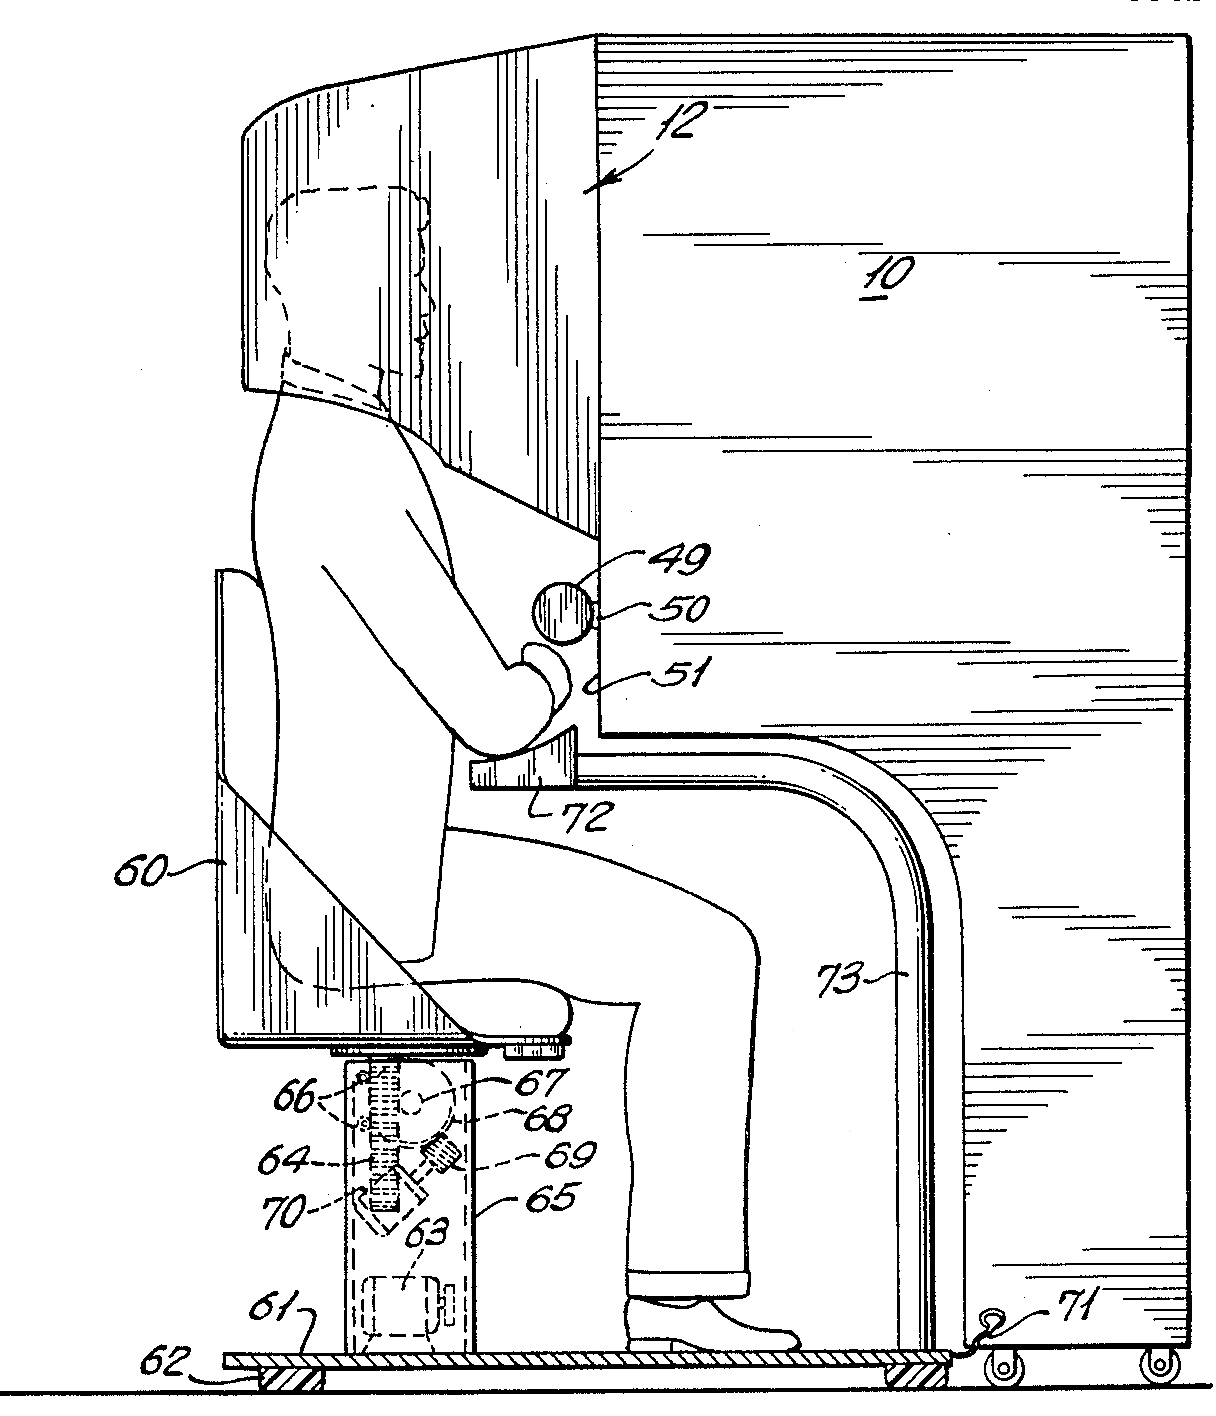
\includegraphics[scale=0.4]{senso.png}
		\caption{Patent Filing for the Sensorama}
		%to ref fig number
		%Figure \ref{fig:block1} shows our blockDiagram.
		\label{fig:sensorama}
	\end{figure}
	The Sensorama  was a huge box that users could stick their head into for what Hellig called the “Cinema of the future”.  It included a fully 3d display, a moving chair (coordinated with the film), and a scent creation device.  It was, perhaps predictably, a failure in terms of revolutionizing cinema, but it did inspire more experiments into virtual reality.  Many of these were military funded, the largest area of development being flight simulators, but in the consumer area the next big leap would come in 1968 with a device called the Sword of Damocles.  It was developed by Ivan Sutherland with help from his student Bob Sproull based on a concept he came up with in 1965, and was the first VR head mounted display.  The device was incredibly bulky and had to be attached to the ceiling so as not to crush the person wearing it, and could only display rudimentary wireframes, but it was the first head mounted display and laid the foundation that our current devices have built upon.  
	Virtual reality remained mostly in labs and research facilities until 1984, when Jaron Lanier created a company called VPL research.  VPL research was one of the first companies to actually attempt to sell VR devices to the world, most notably the dataglove, a peripheral input system that used a glove as input.  This would in turn lead to Mattel creating the Powerglove in 1989, a glove based controller for the NES, one of the first attempts to sell anything virtual reality related to the mass market.  Additionally, VPL research created a more simple head mounted display called the eyephone. Jaron Lanier is also credited with coining the term “Virtual Reality” to describe such devices.  
	\subsubsection{1990-2012}
	The next big breakthrough in consumer virtual reality would come in 1990, with a company called Virtuality Group.  In 1991 they rolled out the first arcade system that relied on virtual reality, known as the 1000 series.[Fig. 2]  
		\begin{figure}[H]
			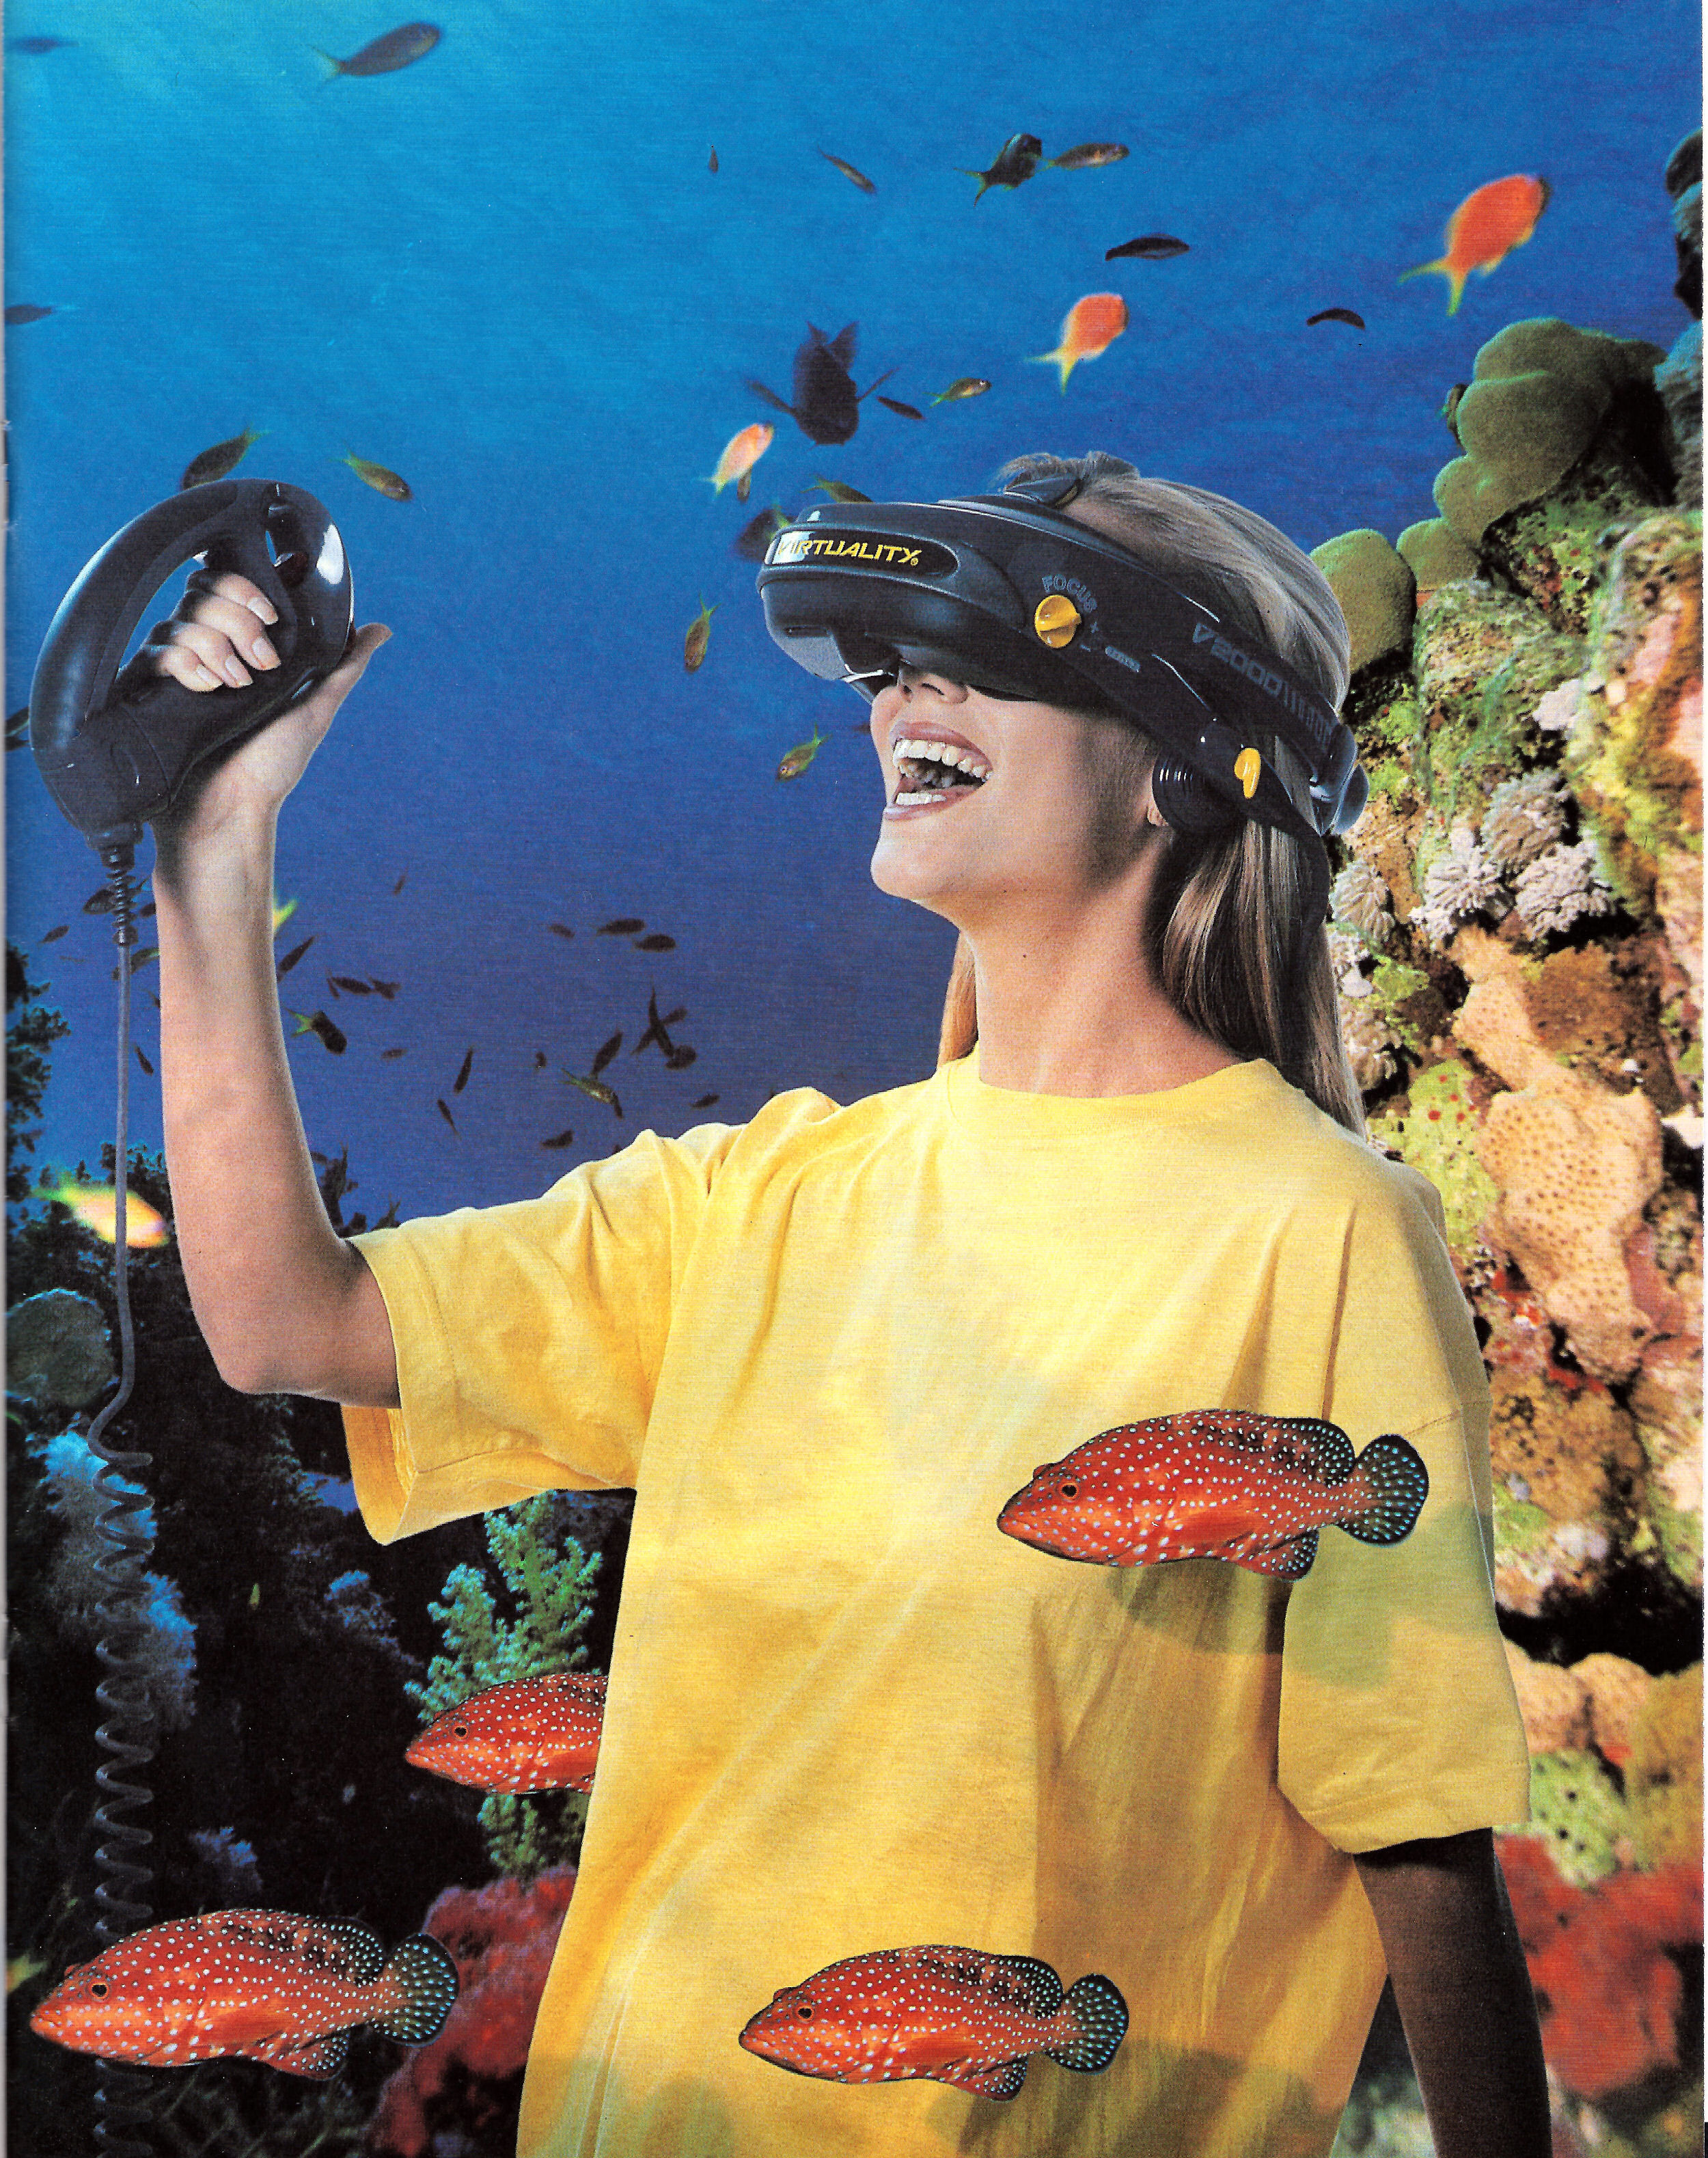
\includegraphics[scale=0.5]{virtuality.jpg}
			\caption{Virtuality Group Advertising}
			%to ref fig number
			%Figure \ref{fig:block1} shows our blockDiagram.
			\label{fig:virtuality}
		\end{figure}It had both stand up and sit down models, all containing a headset that the user would wear.  Along with these arcade machines, Virtuality worked with Sega and Atari to create headsets for their systems, and even tried to develop their own home system.  Nintendo tried to compete as well a virtual reality console called the Virtual Boy.[Fig. 33]
	While impressive and new, all these machines were also comparatively expensive for the player, and also suffered from many of the things VR still struggles with today, like motion sickness and processing power issues.  The games that these systems created also lacked appeal as “games”, instead relying almost entirely on being an innovative new experience.  
	
	The VR market in the 90s turned out to be a bubble waiting to burst, and around 1995 it did.  Ben Delany (founder of Virtuality Group) also blames the internet for the death of VR in the 90s, saying “The mainstream press found other, more exciting things to talk about; especially toward the end of the ’90s when very few of the wild [VR] promises had been fulfilled. People just walked away from it.”.
	VR continued to be grow and be refined, but not at a consumer level.  After the failure of all the major video game companies to create a home market, the industry was declared dead by most analysts and completely ignored.  
	
	However, other fields of development would help create an ecosystem where the VR market could rise again.  The most obvious of these is graphical and processing power.  As computers became more and more powerful and computer graphics became more and more advanced, the idea of placing someone in a virtual world slowly became a feasible concept, as opposed to an idea that people built prototypes after.  On top of this, the huge success of the Nintendo Wii helped develop the field of Motion Controls to the point where people were prepared to consider alternate ways of interacting with a game system.  Lastly, research was still being done on ways to make Virtual Reality hardware and software more powerful.  Jaron Lanier claims that a good portion of what oculus is built on was developed by people working at USC and then posted online, as an open resource.  All of these things created the platform that the Oculus Rift used as a springboard to bring back in a huge way, creating the market that we are going into.
	\subsubsection{Summation}
	
	Before the next section goes into the very recent history of VR, and it’s place in psychology fields, our project can learn some things from the more general history of VR as a consumer product.  The most important and most dangerous thing our team can learn is that our project must not rely on the novelty of virtual reality, it must stand on it’s own merits.  Relying on novelty and the “VR experience” was one of the main things that killed the VR market in 1995.  However, now is also possibly the best time in history for a project like ours, as Virtual Reality has finally hit the point where it is both as popular as it was in the 90s but also has decades of tech development behind it.  Our project is able to leverage not just public support, but years and years of study into how to create virtual worlds.  If we can successfully do that, our project should be in a very good place.
		\begin{figure}[H]
			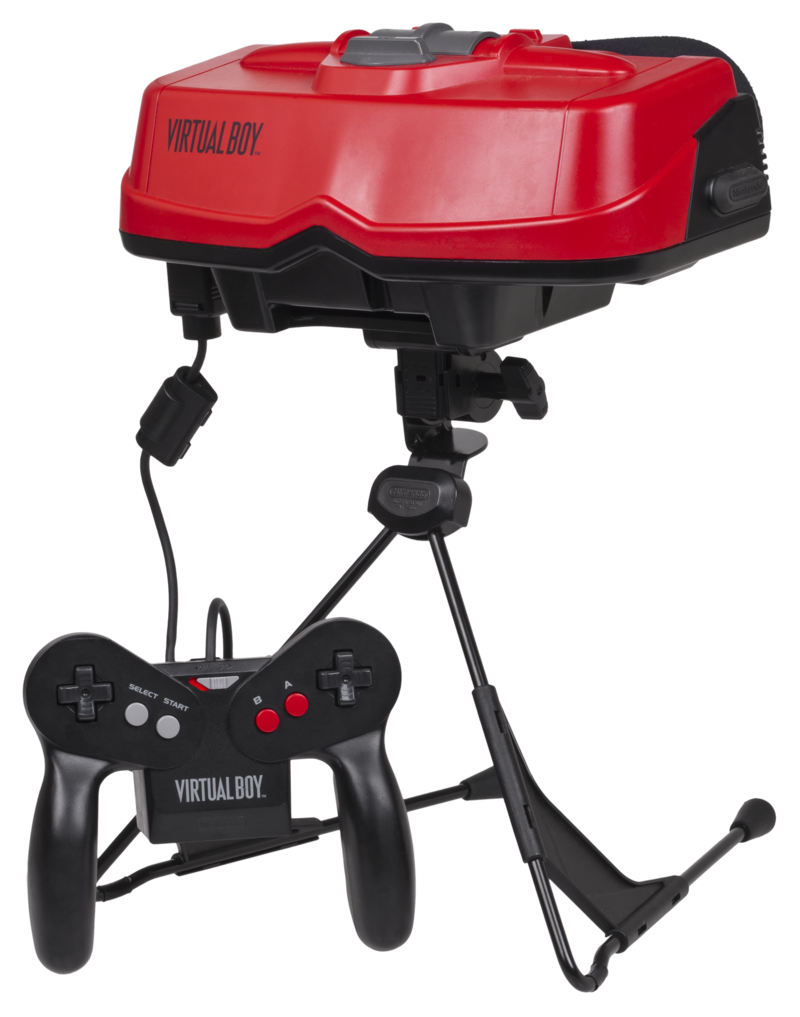
\includegraphics[scale=0.7]{virtualBoy.png}
			\caption{Virtual Boy Advertising}
			%to ref fig number
			%Figure \ref{fig:block1} shows our blockDiagram.
			\label{fig:vBoy}
		\end{figure}

\pagebreak

\subsection{Recent Market History}

\subsubsection{2012: Oculus Rift}

In 2012, a man named Palmer Lucky unveiled a new, consumer grade Virtual Reality device he called the Oculus Rift at the Electronic Entertainment Expo.  2 months later he started a kickstarter to try to raise funds, asking for 250,000 dollars.  This was an unprecedented resurrection of the VR market, relying on modern technology having advanced enough to actually create believable worlds and working hardware.  The project also needed to overcome the stigma that had plagued the market ever since the failure of the Virtual Boy and Virtuality.  1 month later, the project had raised a total of 2,437,429\$ breathing life into a market declared dead for over 15 years.  The kickstarter was a success beyond anyone's imaginings, and would begin a new wave of virtual reality projects.  After raising more money through venture capital and releasing a basic development prototype, om March 25, 2014 Oculus would be acquired for 2 billion dollars by Facebook.  The Virtual Reality market went from dead to 2 billion dollars in only 2 years, and suddenly a large number of companies were interested in VR.

\subsubsection{2014-Present Day: Google, HTC, Sony, and Samsung}

In 2014, 3 different companies would all announce their own attempts at a VR platform.  In March, HTC would announce it's own attempt at virtual reality, named the VIVE, in collaboration with Valve.  This collaboration is the Vive's greatest strength; it has a digital distribution platform (Steam) already at it's disposal.  

Meanwhile, Google announced a strange variation on the VR headset:  they set out plans for a headset users could make with cardboard.  The headset contained a slot to put a smartphone in, and through use of an app the user could have a Virtual Reality headset experience on any modern android equipped phone[Fig. 4].
\begin{figure}[H]
	\centerline{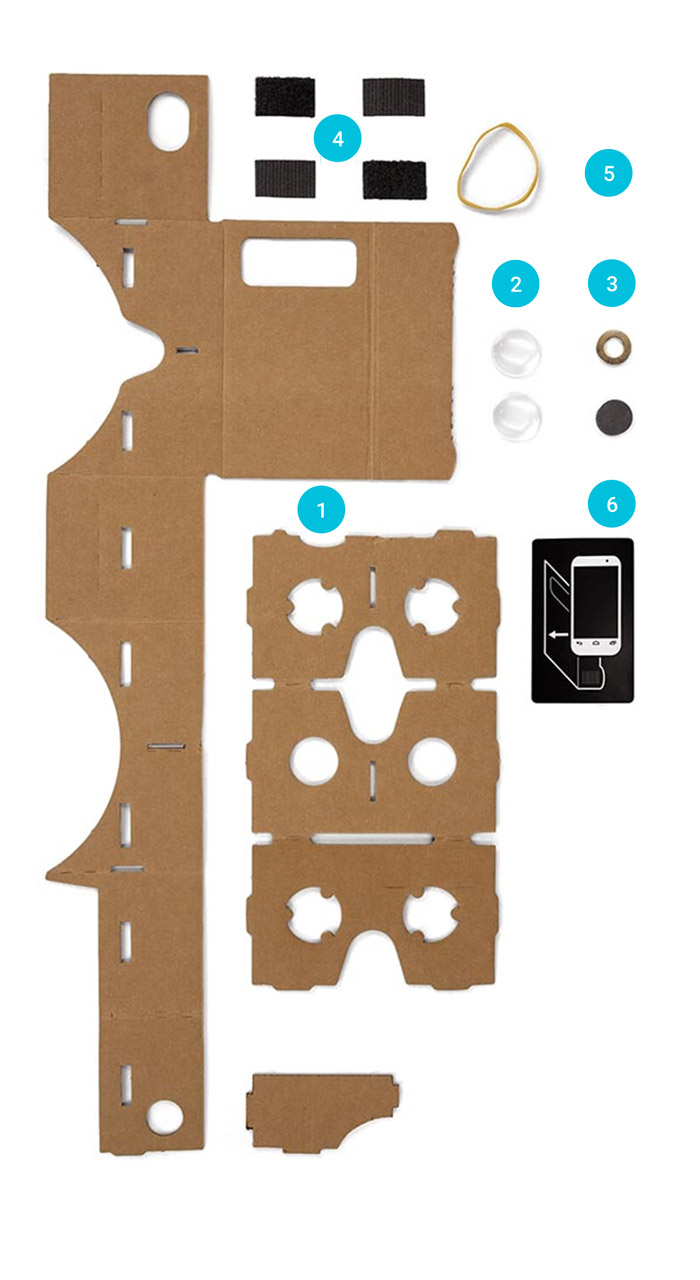
\includegraphics[scale=0.4,angle = 90,keepaspectratio]{cardboard.jpg}}
	\caption{Google Cardboard Diagram}
	%to ref fig number
	%Figure \ref{fig:block1} shows our blockDiagram.
	\label{fig:cardboard}
\end{figure}
Sony would also make an announcment, unveiling the long rumored Project Morpheus at GDC.  Later it would be renamed Playstation VR, and is very heavily reliant on their playstation game console.  Most recently, Oculus announced a collaboration with Samsung to create the Samsung Gear VR.  Like the Google Cardboard, it uses a smartphone as it's display device, however it is a much more specialized device with phones built to work with VR[Fig. 5].

\begin{figure}[H]
	\centerline{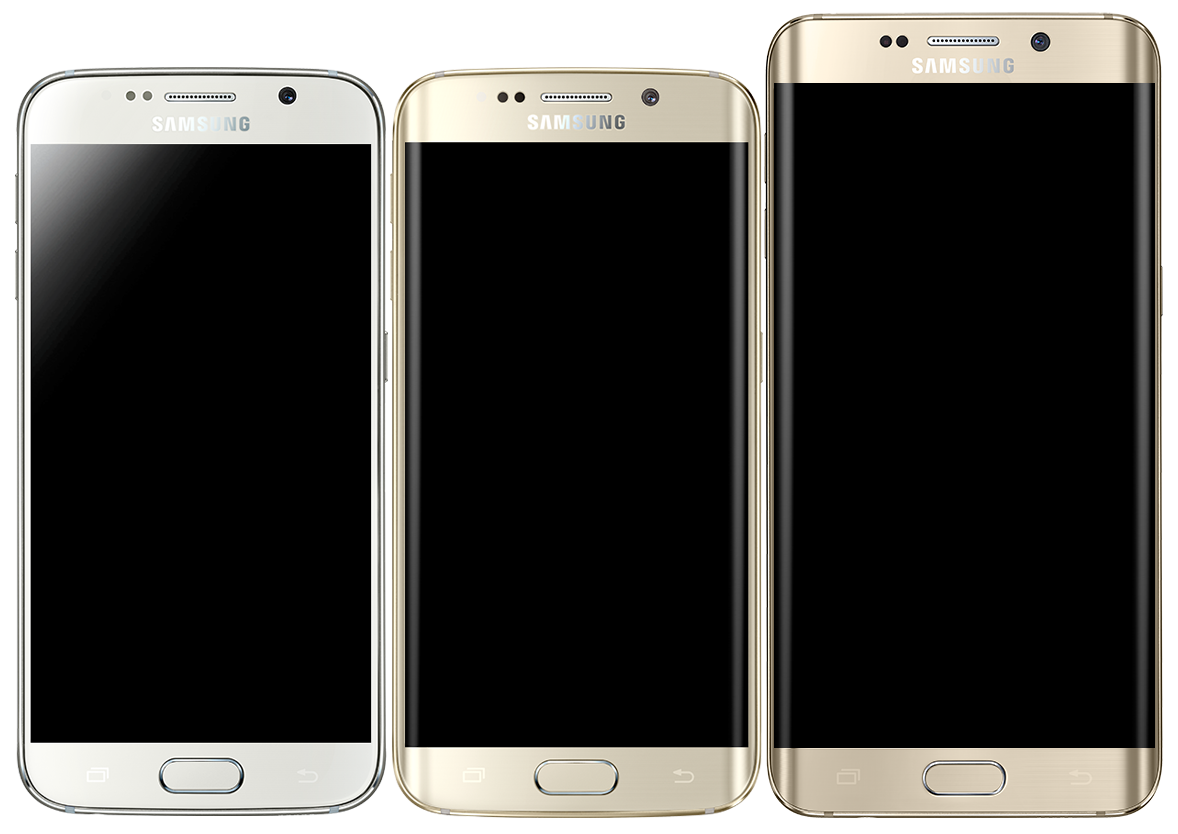
\includegraphics[width=\linewidth,height=\paperheight,keepaspectratio]{galaxy5.png}}
	\caption{Samsung Galaxy S6 series, all compatible with the Gear VR}
	%to ref fig number
	%Figure \ref{fig:block1} shows our blockDiagram.
	\label{fig:samsungGalaxy}
\end{figure}

\subsection{Market Future}
\subsubsection{Statistics}

Current predictions for the VR market are overall positive.  The next couple of pages [Fig 6-8] are a number of statistics and surveys showing predictions for the growth of the VR field over the next 4-5 years.  Each contains a description and source.  Following this section will be a conclusion, wrapping up both the research on recent VR companies and these statistics.

\begin{figure}[H]
	\centerline{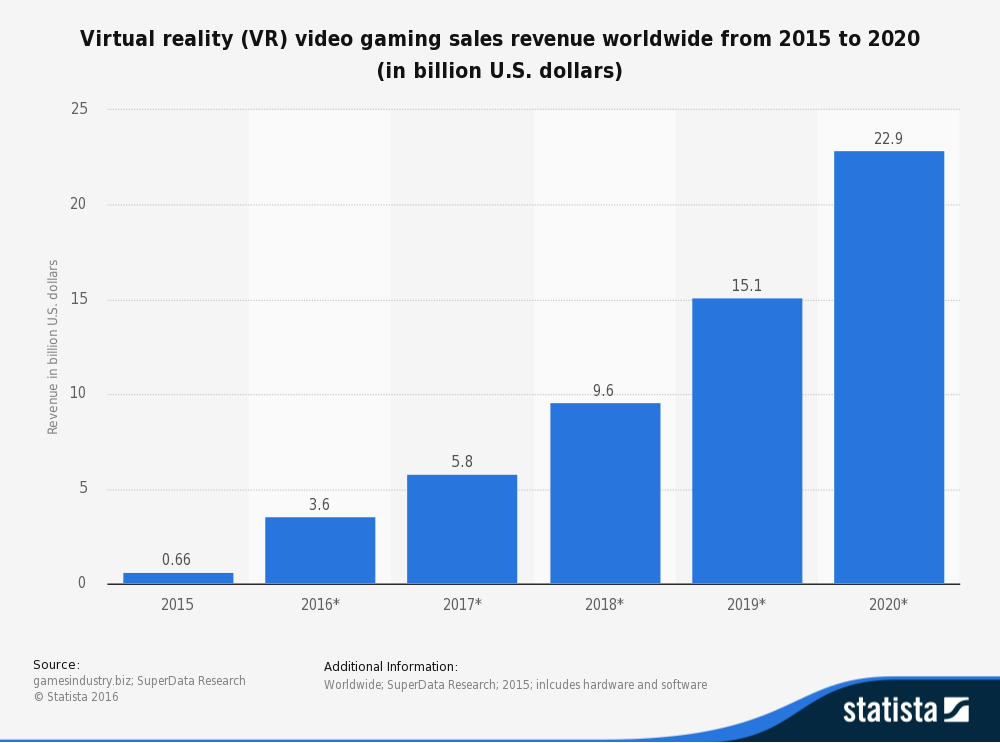
\includegraphics[scale = 0.3]{statMon2.png}}
	\caption{Prediction of the virutal reality revenue through 2020.  Obtained through Statistia.  Source: Superdata Research}
	%to ref fig number
	%Figure \ref{fig:block1} shows our blockDiagram.
	\label{fig:virRevenue}
\end{figure}

\begin{figure}[H]
	\centerline{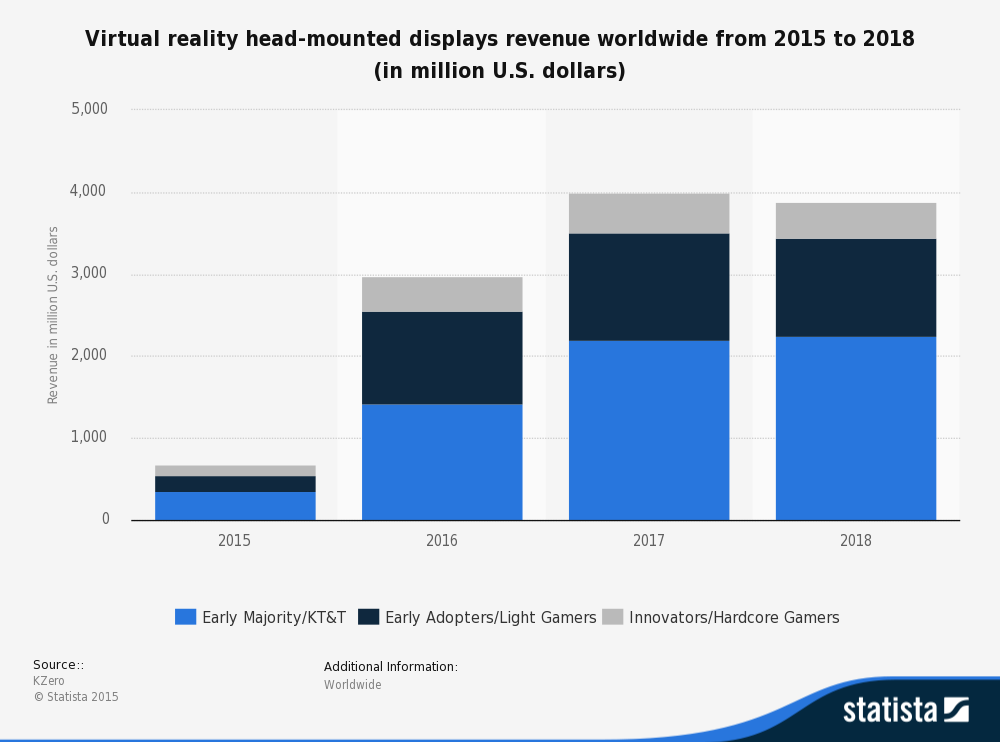
\includegraphics[scale = 0.3]{statMon.png}}
	\caption{Prediction of the Head Mounted Display Revenue through 2018.  Obtained through Statistia.  Source: KZero survey}
	%to ref fig number
	%Figure \ref{fig:block1} shows our blockDiagram.
	\label{fig:moneyStats}
\end{figure}

\begin{figure}[H]
	\centerline{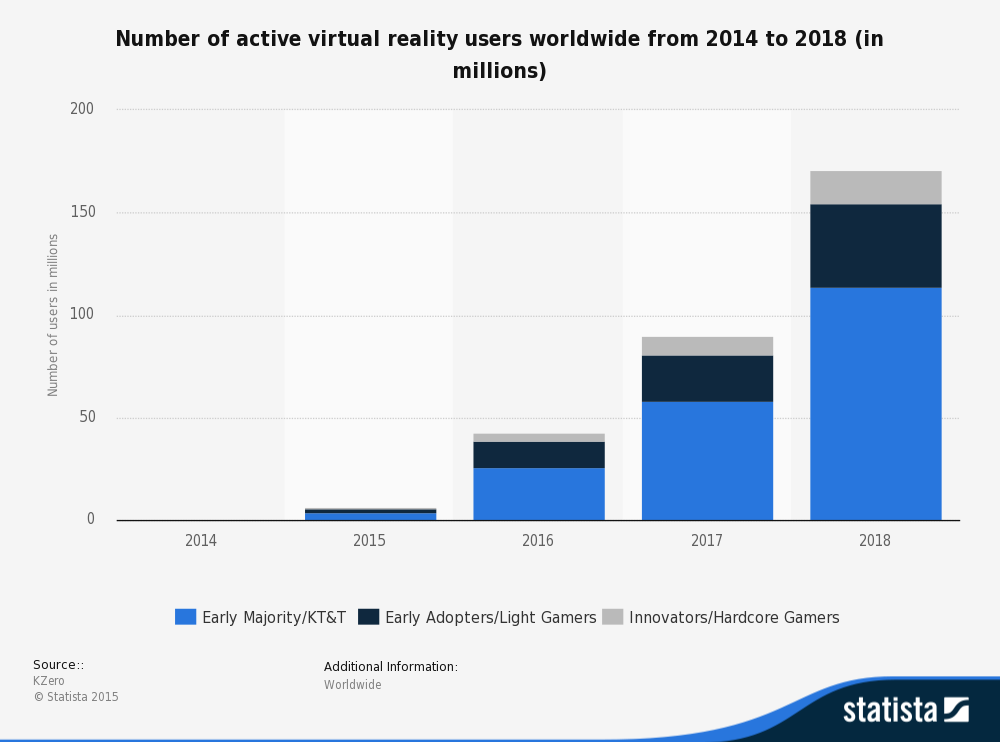
\includegraphics[scale = 0.25]{statsUsers.png}}
	\caption{Prediction of the virutal reality user acceptance through 2018.  Obtained through Statistia.  Source: KZero survey}
	%to ref fig number
	%Figure \ref{fig:block1} shows our blockDiagram.
	\label{fig:userStats}
\end{figure}

\begin{figure}[H]
	\centerline{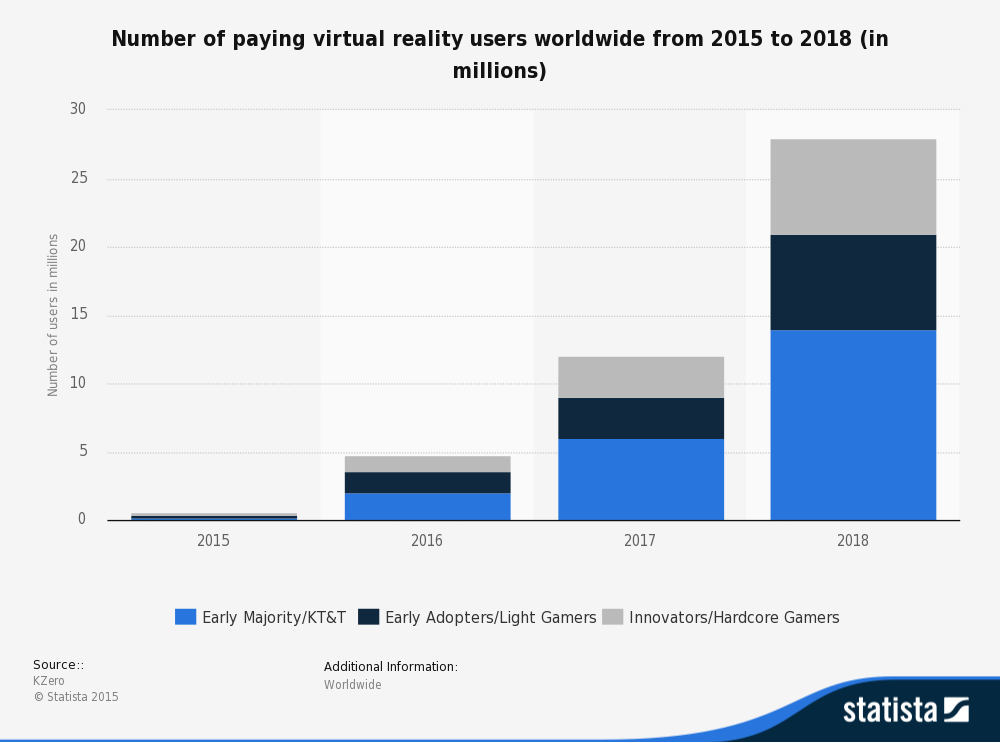
\includegraphics[scale = 0.25]{statPay.png}}
	\caption{Prediction of the paying virtual reality users through 2018.  Obtained through Statistia.  Source: KZero survey}
	%to ref fig number
	%Figure \ref{fig:block1} shows our blockDiagram.
	\label{fig:moneyStats}
\end{figure}
\subsubsection{Conclusion}
\pagebreak
\subsection{VR Headset Options and Technical Capabilities}
\subsubsection{Oculus Rift Consumer Version}
\begin{itemize}
	\item Resolution: 2160 x 1200
	\item Refresh Rate: 90 Hz (11 ms !!)
	\item Latency: 20ms
	\item Recommended CPU: Intel i5-4590 or equivalent
	\item Recommended GPU: NVIDIA GTX 970 / AMD 290 
	\item Recommended RAM: 8GB
	\item Positional Tracking: IR Camera Sensor (5 x 11 feet)
	\item Controls: Oculus Touch (not included)
	\item Release Date: Q1 2016 (Delayed)
	\item Manufacturer: Oculus VR
	\item Unity Support: Yes
	\item OS Cross Platform: Windows and Android only. (Oculus Home Dependent)
	\item Cost: \$599
\end{itemize}
\begin{figure}[H]
	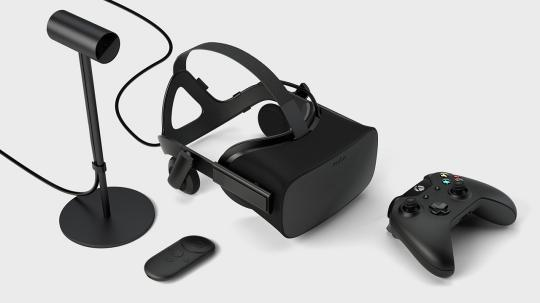
\includegraphics[width=\linewidth,height=\paperheight,keepaspectratio]{cv.jpg}
	\caption{Oculus Rift Consumer Version}
	%to ref fig number
	%Figure \ref{fig:block1} shows our blockDiagram.
	\label{fig:RiftCVImg}
	\end{figure}
	\pagebreak
\subsubsection{Oculus Rift Dev Kti 2}
\begin{itemize}
	\item Resolution: 1920 x 1080
	\item Refresh Rate: 75 Hz (13 ms)
	\item Latency: 20-40ms
	\item Recommended CPU: Intel i5-4590 or equivalent
	\item Recommended GPU: NVIDIA GTX 970 / AMD 290 
	\item Recommended RAM: 8GB
	\item Positional Tracking: IR Camera Sensor (5 x 11 feet)
	\item Controls: Oculus Touch (not included)
	\item Release Date: July 2014
	\item Manufacturer: Oculus VR
	\item OS Cross Platform: Windows and Android only. (Oculus Home Dependent)
	\item Unity Support: Yes
	\item Cost: \$350
\end{itemize}
\begin{figure}[H]
	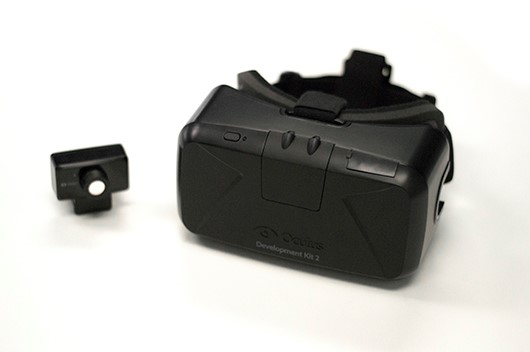
\includegraphics[width=\linewidth,height=\paperheight,keepaspectratio]{dk2.jpg}
	\caption{Oculus Rift Dev Kti 2}
	%to ref fig number
	%Figure \ref{fig:block1} shows our blockDiagram.
	\label{fig:Riftdk2Img}
	\end{figure}
	\pagebreak
\subsubsection{Oculus Rift Dev Kit 1}
\begin{itemize}
	\item Resolution: 1200 x 800
	\item Refresh Rate: 60 Hz (16 ms)
	\item Latency: 50-60ms
	\item Recommended CPU: Lower Spec (Early Prototype)
	\item Recommended GPU: Lower Spec (Early Prototype)
	\item Recommended RAM: 4GB
	\item Positional Tracking: No
	\item Controls: Oculus Touch (not included) 
	\item Release Date: August 2012 (Kickstarter)
	\item Manufacturer: Oculus VR
	\item Cross Platform: Windows and Android only. (Oculus Home Dependent)
	\item Unity Support: Yes
	\item Cost: \$300
\end{itemize}
	\begin{figure}[H]
	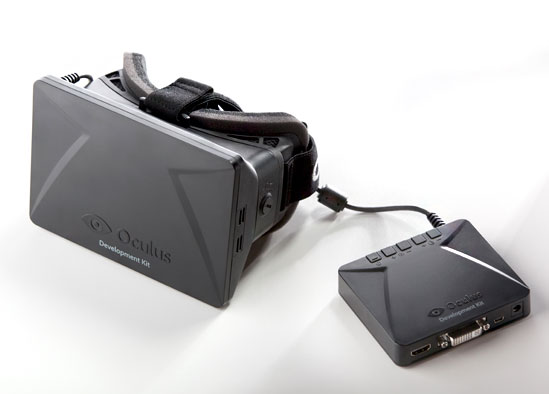
\includegraphics[width=\linewidth,height=\paperheight,keepaspectratio]{dk1.jpg}
	\caption{Oculus Rift Dev Kit 1}
	%to ref fig number
	%Figure \ref{fig:block1} shows our blockDiagram.
	\label{fig:Riftdk1Img}
	\end{figure}
	\pagebreak
\subsubsection{Samsung Gear VR}
	Supported Phones Include the Samsung Galaxy: Note5, S6, S6 edge, S7, S7 edge  
	\begin{itemize}
	  \item Resolution: 2560 X 1440 (Quad HD phone screen)
	  \item Refresh Rate: 60 Hz (16 ms)
	  \item Latency: 50-60ms
	  \item Recommended CPU: Phone Dependent
	  \item Recommended GPU: Phone Dependent
	  \item Recommended RAM: Phone Dependent
	  \item Positional Tracking: No
	  \item Controls: Touch pad, back button, volume controls
	  \item Release Date: November 2015
	  \item Manufacturer: Samsung, With technology by Oculus VR
	  \item Cross Platform: Windows and Android only. (Oculus Home Dependent)
	  \item Unity Support: Yes
	  \item Cost: \$99
	\end{itemize}
	\begin{figure}[H]
	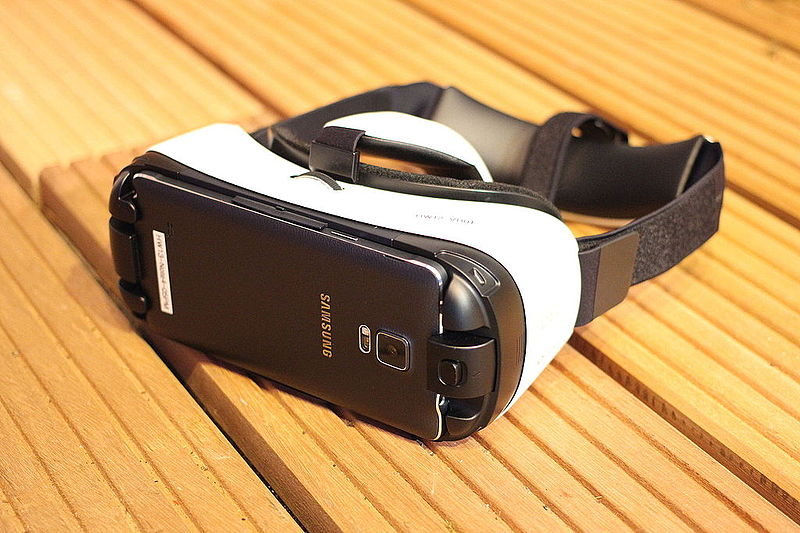
\includegraphics[width=\linewidth,height=\paperheight,keepaspectratio]{gear.jpg}
	\caption{Samsung Gear VR}
	%to ref fig number
	%Figure \ref{fig:block1} shows our blockDiagram.
	\label{fig:GearImg}
	\end{figure}
	\pagebreak
\subsubsection{HTC Vive}
	\begin{itemize}
	  \item Resolution: 2160 x 1200
	  \item Refresh Rate: 90 Hz (11 ms)
	  \item Latency: 22ms
	  \item Recommended CPU: Intel i5-4590 or equivalent
	  \item Recommended GPU: NVIDIA GTX 970 / AMD 280 
	  \item Recommended RAM: 4GB
	  \item Positional Tracking: IR Camera Sensor (15 x 15 feet)
	  \item Controls: Motion Controllers (included) (similar to Occulus Touch)  
	  \item Release Date: Q1 2016 (Delayed)
	  \item Manufacturer: HTC, With technology by Valve Corporation
	  \item Cross Platfrom: Valve OpenGL Mesa support/ SteamVR support on Linux soon hopefully
	  \item Unity Support: Yes
	  \item Cost: \$799
	\end{itemize}
	\begin{figure}[H]
	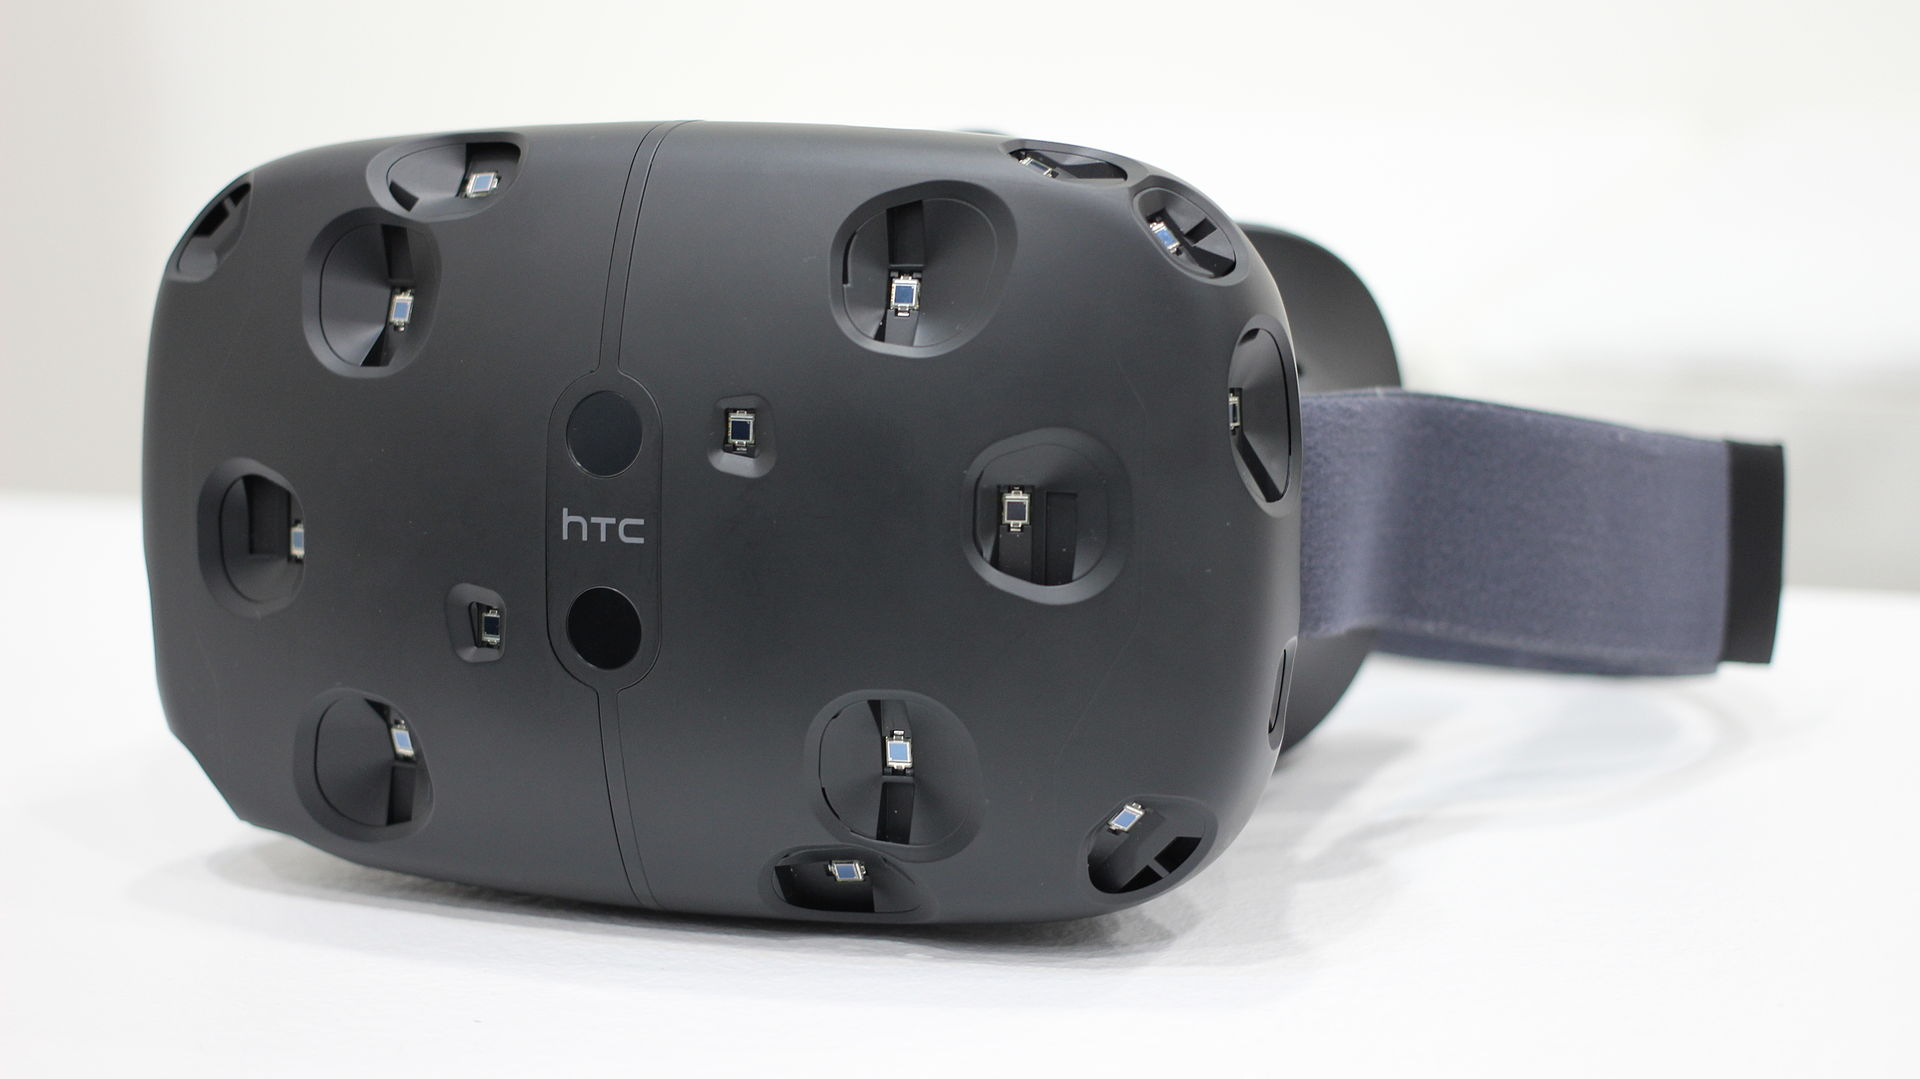
\includegraphics[width=\linewidth,height=\paperheight,keepaspectratio]{vive.jpg}
	\caption{HTC Vive Headset}
	%to ref fig number
	%Figure \ref{fig:block1} shows our blockDiagram.
	\label{fig:ViveImg}
	\end{figure}
	\pagebreak
\subsubsection{PS4 Morpheus}
\begin{itemize}
  \item Resolution: 3840 x 1080 
  \item Refresh Rate: 120 Hz (8 ms)
  \item Latency: 18ms
  \item Recommended CPU: PS4
  \item Recommended GPU: PS4
  \item Recommended RAM: PS4
  \item Positional Tracking: Playstation Camera area ~(18 x 12 feet)
  \item Controls: Playstation Move Controllers (not included)
  \item Release Date: Q1 2016 (Delayed)
  \item Manufacturer: Sony
  \item Cross Platfrom: No
    \item Unity Support: Yes
  \item Unity Support: Yes
  \item Cost: \$399
\end{itemize}
\begin{figure}[H]
	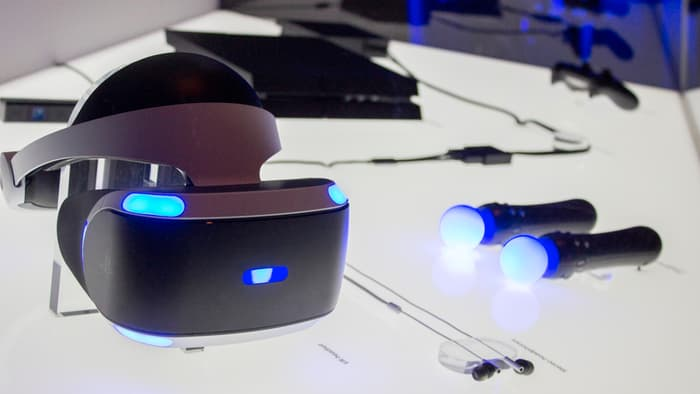
\includegraphics[width=\linewidth,height=\paperheight,keepaspectratio]{morpheus.jpg}
	\caption{Playstation VR}
	%to ref fig number
	%Figure \ref{fig:block1} shows our blockDiagram.
	\label{fig:psvrImg}
\end{figure}
	\pagebreak
	
\pagebreak
\subsection{VR Peripheral Options}
precision, inputs, basic info
\subsubsection{Leap Motion}
\begin{itemize}
	\item Using Leap Motion on a PC is viable in Unity and very well supported, however using Leap Motion and the Gear VR simultaneously on Android is not feasible, this is due to the high level of processing required to
	handle the areas tracked by the leap sensor. 
	\item The primary support is designed to work with the Oculus rift, and unity is supported by the Leap SDK. Making it a powerful useful sensor for hand tracking. The 
	Leap motion is supported on the Oculus DK2 and the new CV (consumer release). 
\end{itemize}
\begin{figure}[H]
	\centerline{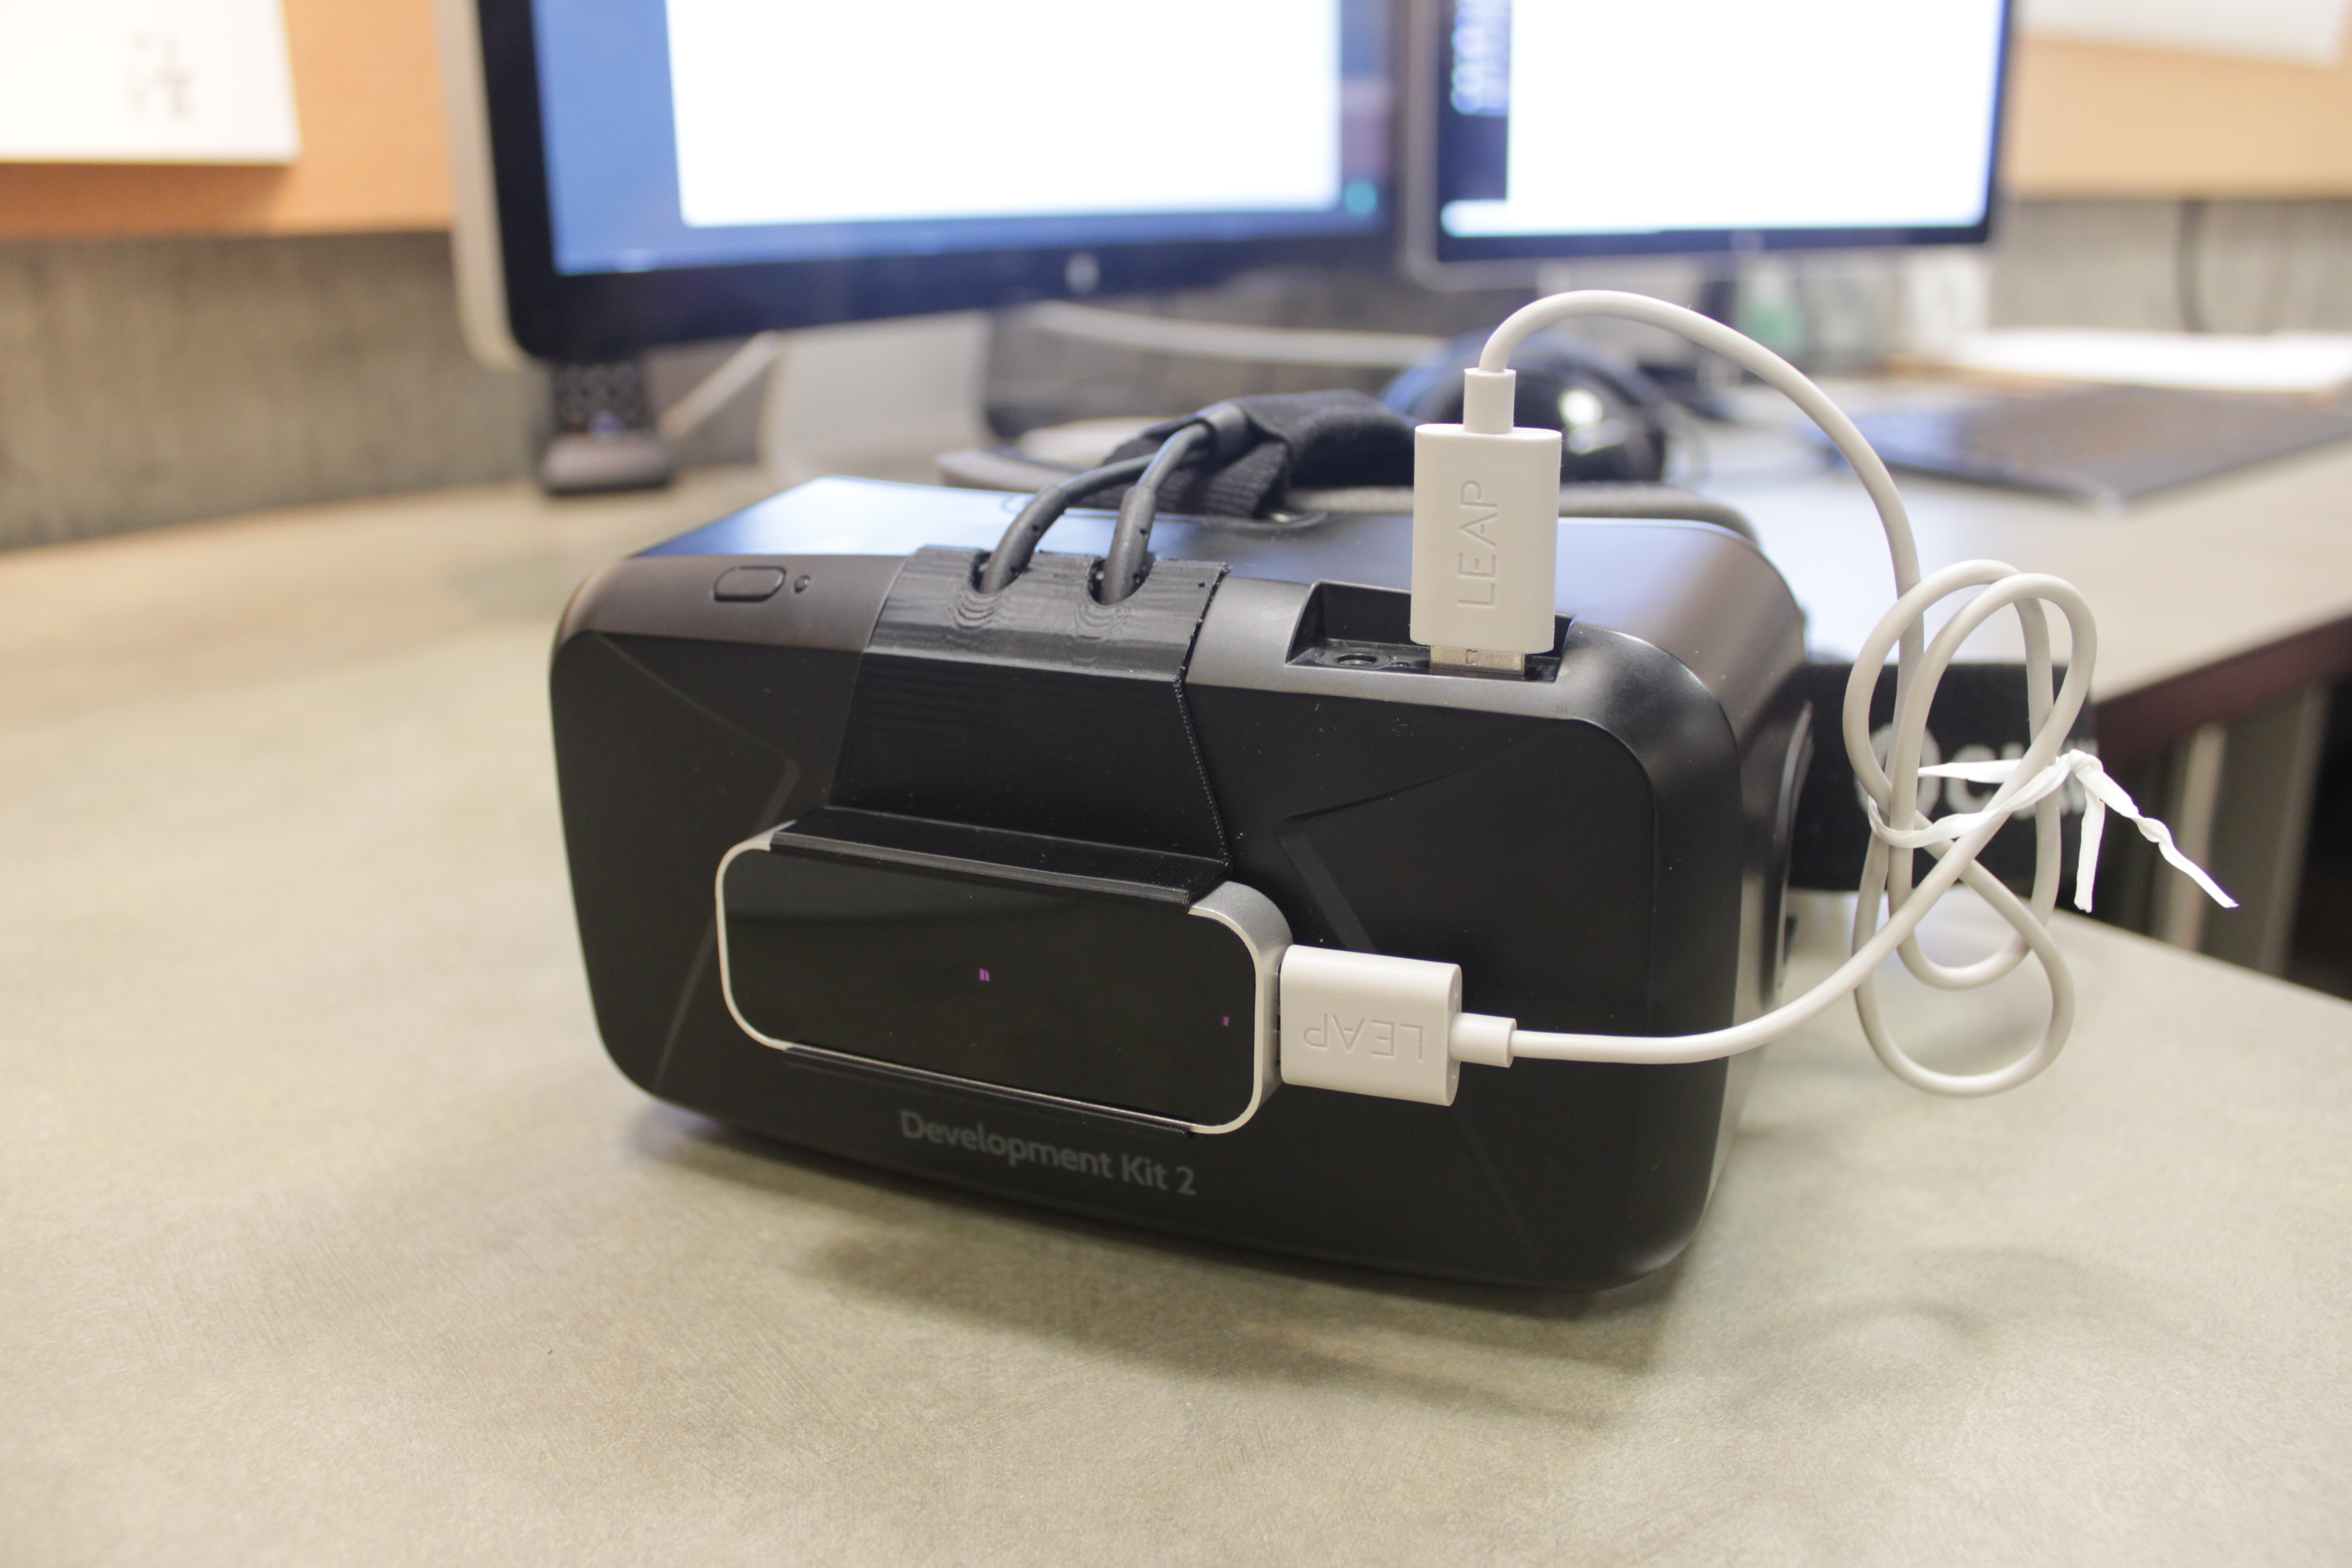
\includegraphics[scale= 0.08]{leap.jpg}}
	\caption{Playstation VR}
	%to ref fig number
	%Figure \ref{fig:block1} shows our blockDiagram.
	\label{fig:leapImg}
\end{figure}
	
	
\subsubsection{Red Samurai Bluetooth Controller}
	A cheap, \$8 bluetooth controller, that pairs very well with the Gear VR on Android, this would be allow the user to move around the scene as we would be unable to get the other Peripherals to work with the phone.
\pagebreak
\subsection{Movement Tracking Cameras}
\subsubsection{Microsoft Kinect 1}
\begin{itemize}
  \item Resolution: 640 X 480
  \item Refresh Rate: 33 Hz (30 FPS)
  \item Max Depth: 12 feet
  \item Release Date: August 2010 
  \item Manufacturer: Microsoft
  \item Cross Platform: Yes
  \item Unity Support: Yes
  \item Skeleton Joints:: 26
  \item Horizontal FOV: 57 Degrees
  \item Vertical FOV: 43 Degrees
  \item Pixels Per Degree: 5 X 5
  \item Technique: Structured Light Patterns
  \item Cost: Acquired, Not widely available, ~\$40
\end{itemize}
\begin{figure}[H]
	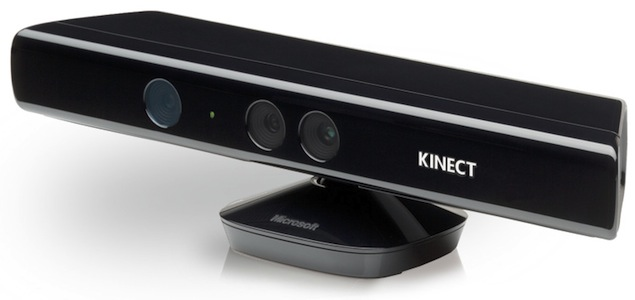
\includegraphics[width=\linewidth,height=\paperheight,keepaspectratio]{kinect1.jpg}
	\caption{Kincet 1 Camera}
	%to ref fig number
	%Figure \ref{fig:block1} shows our blockDiagram.
	\label{fig:k1Cam}
	\end{figure}
	\pagebreak
	\subsubsection{Microsoft Kinect 2}
\begin{itemize}
  \item Resolution: 1920 X 1080
  \item Refresh Rate: 33 Hz (30 FPS)
  \item Max Depth: 12 feet
  \item Release Date: August 2010 
  \item Manufacturer: Microsoft
  \item Cross Platfrom: Yes
  \item Skeleton Joints: 26
  \item Horizontal FOV: 70 Degrees
  \item Vertical FOV: 60 Degrees
  \item Pixels Per Degree: 7 X 7
  \item Technique: Time of Flight
  \item Cost: \$99
\end{itemize}
\begin{figure}[H]
	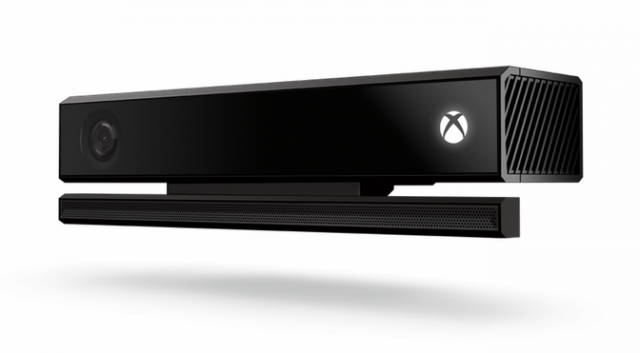
\includegraphics[width=\linewidth,height=\paperheight,keepaspectratio]{kinect2.jpg}
	\caption{Kincet 2 Camera}
	%to ref fig number
	%Figure \ref{fig:block1} shows our blockDiagram.
	\label{fig:k2Cam}
	\end{figure}
	\pagebreak
	
\subsubsection{Comparison of Kinect Systems}
\textbf{(Figure \ref{fig:kimg})} shows the increased fidelity and quality of the captured image on the kinect 2.
\begin{figure}[H]
	\centerline{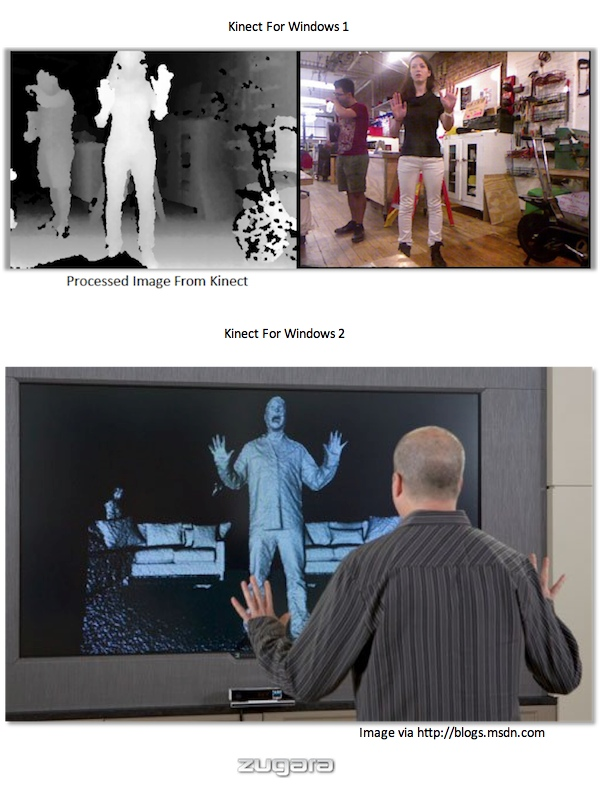
\includegraphics[scale=0.5]{kinectImg.jpg}}
	\caption{Kincet 2 Camera}
	%to ref fig number
	%Figure \ref{fig:block1} shows our blockDiagram.
	\label{fig:kimg}
	\end{figure}
	\pagebreak	
	
\subsubsection{Oculus Rift DK2+ Camera}
\begin{itemize}
  \item Resolution: 752×480
  \item Refresh Rate: 16 Hz (60 FPS)
  \item Max Depth: ?
  \item Release Date: July 2014
  \item Manufacturer: Oculus Rift
  \item Cross Platfrom: No
  \item Skeleton Joints: Heaset Position
  \item Technique: IR LED Pattern Recognition
  \item Cost: Included With Headset
\end{itemize}
\begin{figure}[H]
	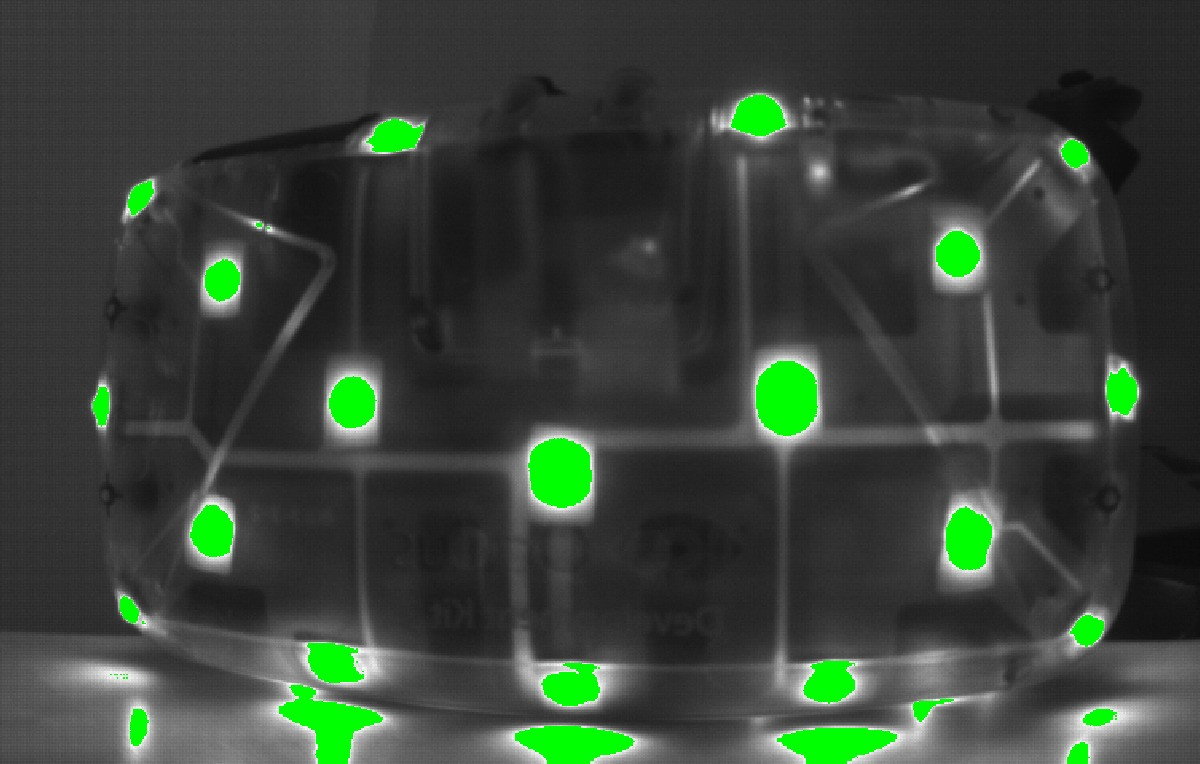
\includegraphics[width=\linewidth,height=\paperheight,keepaspectratio]{riftIR.jpg}
	\caption{Rift Sensor IR}
	%to ref fig number
	%Figure \ref{fig:block1} shows our blockDiagram.
	\label{fig:riftCam}
	\end{figure}
	\pagebreak
	\subsubsection{HTC Vive Lighth House Sensors}
\begin{itemize}
  \item Resolution: 752×480
  \item Refresh Rate: 16 Hz (60 FPS)
  \item Max Depth: ?
  \item Release Date: July 2014
  \item Manufacturer: Oculus Rift
  \item Cross Platfrom: No
  \item Skeleton Joints: Heaset Position
  \item Horizontal FOV: NA
  \item Vertical FOV: NA
  \item Pixels Per Degree: NA
  \item Technique: 360 Laser / LED full room scanning 
  \item Cost: Included With Headset
\end{itemize}
\begin{figure}[H]
	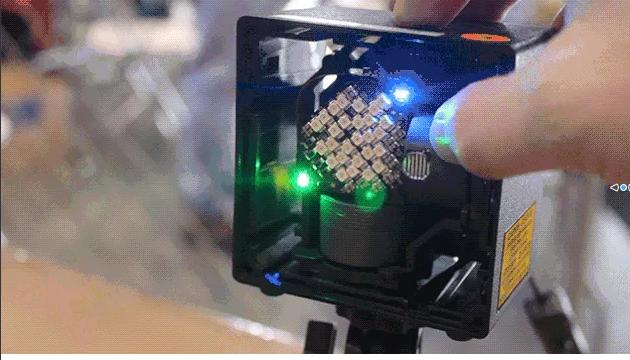
\includegraphics[width=\linewidth,height=\paperheight,keepaspectratio]{viveLight.jpg}
	\caption{HTC Lighthouse Sensor}
	%to ref fig number
	%Figure \ref{fig:block1} shows our blockDiagram.
	\label{fig:viveCam}
	\end{figure}
	\pagebreak

\subsection{Compnay Histories}
%rift startup, other infos here...

\subsection {Psychology research}
This Section will discuss various psychological areas of our project including warnings, limitations, trends, other successful tests, and specifics about different phobias or disorders 
that we are researching. 
%http://www.ncbi.nlm.nih.gov/pmc/articles/PMC4538594/
\paragraph{DSM Cautionary Statement}  ~\\
Any cited DSM excepts ofter include this statement as a disclaimer. \cite{dsmCaution}
\begin{itemize}

\item The specified diagnostic criteria for each mental disorder are offered as guidelines for making diagnoses, because it has been demonstrated that 
the use of such criteria enhances agreement among clinicians and investigators. The proper use of these criteria requires specialized clinical
training that provides both a body of knowledge and clinical skills. 

\item These diagnostic criteria and the DSM-IV Classification of mental disorders reflect a consensus of current formulations of evolving knowledge in
our field. They do not encompass, however, all the conditions for which people may be treated or that may be appropriate topics for research efforts. 

\item The purpose of DSM-IV is to provide clear descriptions of diagnostic categories in order to enable clinicians and investigators to diagnose, communicate
about, study, and treat people with various mental disorders. It is to be understood that inclusion here, for clinical and research purposes, of a diagnostic
category such as Pathological Gambling or Pedophilia does not imply that the condition meets legal or other nonmedical criteria for what constitutes mental disease,
mental disorder, or mental disability. The clinical and scientific considerations involved in categorization of these conditions as mental disorders may not be wholly 
relevant to legal judgments, for example, that take into account such issues as individual responsibility, disability determination, and competency.
\end{itemize}
\pagebreak
\subsubsection{DSM Criteria for Specific Phobias}
\paragraph{DSM IV}~\\
(cautionary statement) 
\begin{itemize}
\item Marked and persistent fear that is excessive or unreasonable, cued by the presence or anticipation of a specific object or situation (e.g., flying, heights, animals, receiving an
injection, seeing blood). 
\item Exposure to the phobic stimulus almost invariably provokes an immediate anxiety response, which may take the form of a situationally bound or situationally predisposed Panic Attack. 
Note: In children, the anxiety may be expressed by crying, tantrums, freezing, or clinging. 
\item  The person recognizes that the fear is excessive or unreasonable. Note: In children, this feature may be absent. 
\item The phobic situation(s) is avoided or else is endured with intense anxiety or distress. 
\item The avoidance, anxious anticipation, or distress in the feared situation(s) interferes significantly with the person's normal routine, occupational (or academic) functioning, or
social activities or relationships, or there is marked distress about having the phobia. 
\item In individuals under age 18 years, the duration is at least 6 months.
\item The anxiety, Panic Attacks, or phobic avoidance associated with the specific object or situation are not better accounted for by another mental disorder, such as Obsessive-
Compulsive Disorder (e.g., fear of dirt in someone with an obsession about contamination), Posttraumatic Stress Disorder (e.g., avoidance of stimuli associated with a severe stressor),
Separation Anxiety Disorder (e.g., avoidance of school), Social Phobia (e.g., avoidance of social situations because of fear of embarrassment), Panic Disorder with Agoraphobia, or 
Agoraphobia Without History of Panic Disorder. \cite{dsmPhobia}
\end{itemize}

\paragraph{Specific types:} 
\begin{itemize}
\item Animal Type
\item Natural Environment Type (e.g., heights, storms, water) 
\item Blood-Injection-Injury Type 
\item Situational Type (e.g., airplanes, elevators, enclosed places) 
\item Other Type (e.g., phobic avoidance of situations that may lead to choking, vomiting, or contracting an illness; in children, avoidance of loud sounds or costumed characters)
\end{itemize}
\pagebreak
\subsubsection{Examples of Success}
For example, 12 studies tested the effects of virtual reality on stroke recovery. 5 of these studies showed patients who played virtual reality games were about 4.9 times more likely to improve their upper body strength than those who received the standard therapy, while the other 7  studies showed a 14.7 percent improvement, on average, in patients' grip strength and a 20 percent improvement in patient's ability to perform standard tasks.\cite{stroke1}
\pagebreak
\subsection{Module 1 Fear of Heights}
The fear of heights module will be built around the success of past and present research. Fear of heights, referred to as acrophobia, is a popular target for studying the impact of virtual reality on treatment. For this scene the user will be at the ground floor of a 50 story building and may ride a glass elevator up to any desired floor. Past experiments and studies on using virtual reality for acrophobia treatment have lacked high quality graphical experiences which can detract from the immersionn. Our background will feature a detailed cityscape to increase the realism the user experiences and likely increase the effectiveness of treatment.
\pagebreak
\subsection{Module 2 Speech Anxiety Simulator}
Speech Anxiety is the next issue we wish to treat with virtual reality therapy. As another popular target of VR therapy research, speech anxiety has several successful examples. In our implementation the user will be able to configure the environment in which they practice public speaking to better suit their needs and deliver a more personal experience. We will begin with a classroom environment with chair spots which the user can place different students into and configure their actions such as sleeping, focused, or texting. As a stretch goal for this module we will implement more varying environments like a conference room and a stage.
\pagebreak
\subsection{Module 3 Calm Environment} % SO HYPED!!!
This module will feature a calming environment that will help patients with stress or anxiety relax in a calming peaceful environment. This environment will have random terrain which will have chunks 
that are procedurally generated while the user moves throughout the scene.  The art style/ graphic design for this project is inspired by an indie game called proteus \textbf{(See Figure \ref{fig:proteus})}. 
It will feature simple generated terrains that form a  peaceful landscape which the user can move throughout with various plants or natural features that decorate the scene. 
Some configuration options for this scene include different biomes or selecting what models are loaded or how the scene looks in general. 

\begin{figure}[H]
	\centerline{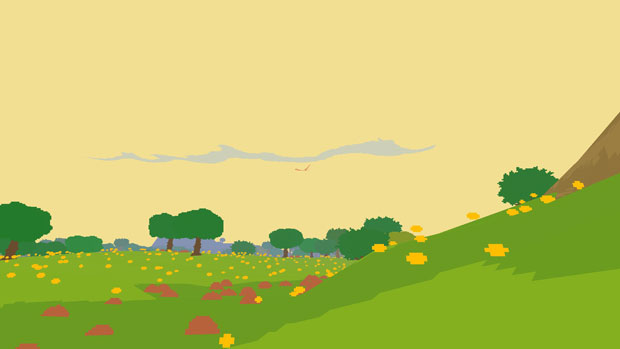
\includegraphics[scale= 0.4]{proteus.jpg}}
	\caption{Proteus Picture}
	%Figure \ref{fig:gpgpuImg} shows our blockDiagram.
	\label{fig:proteus}
	\end{figure}
\subsubsection{Design Concerns}
Some solutions include some premade plug-ins that generate some terrains, on the CPU with possibly some GPU acceleration, however we would like to try and generate our own
terrain with Compute Shader provided in Unity.


\paragraph{Some factors that may limit our ability to do this include:}
\begin{itemize}
\item Access to some features related to direct pipeline which only comes with the Professional Version.
\item The efficiency of our generation and mapping algorithms on the GPU.
\item The already heavy load of meeting rendering demands of release level VR headsets which require a large frame buffer for two screens which each require different OpenGL rendering passes.
\item Most of these issues will be handled by Unity for most scenes but if we want to do any mapping on the fly we will have to meet these rendering/ processing time lines for our compute operations, 
and deal with the extra processing overhead for the GPU while making sure we can run the VR with decent settings and frame rates. 
\item We Will pick the best option for the terrain that provides the best immersion for the user and performance.
\end{itemize}
% https://scrawkblog.com/category/directcompute/
% http://answers.unity3d.com/questions/162096/gpu-programming-with-unity.html
\pagebreak
\subsubsection{GPGPU Research Outline}
Any generated terrain Unity supports compute shaders which are written in Direct X HLSL, and allow the application to do computations on the GPU for
these terrain calculations. These compute shaders allow the application to do most of the heavy computations on the GPU which provides massive speedups compared to the a CPU implementation.
\paragraph{This Section will discuss the following:}
\begin{itemize}
	\item GPU Overview 
	\begin{itemize}
		\item GPGPU Overview
		\item GPGPU processing model
		\item GPU Architecture
	\end{itemize}
	\item Unity Compute Shader/ GPU Processing Features
	\begin{itemize}
		\item Compute Shader Support
		\item Cross Platform Support
		\item Asynchronous Buffer Synchronization
		\item Unity Rendering Pipeline Features
		\item Advanced Compute Shader GPGPU Features
	\end{itemize}
	\item Overall Analysis On GPU Compute Shaders
\end{itemize}
\pagebreak
\subsubsection{General-purpose computing on graphics processing units (GPGPU)}
GPGPU programming is a growing option for parallel processing applications that work over large data sets. Some common uses include image or media processing and 
performing mathematical computations over linear systems or large sets. Many modern GPUs offer many benefits in processing with the high number of cores that can operate on data 
in Single Instruction Multiple Data (SIMD) and Multiple Instruction Multiple Data (MIMD) fashions. For example, one group of data can be processed with the same instruction in parallel 
and the GPU can have multiple groups scheduled at the same time. The basic unit of execution on a GPU (the compute shader or kernel) is run in parallel and scheduled by the GPU execution context
and the commands are setup and issued by the cpu application in a queue fashion, some execution can be synched to wait for other kernels to complete or can be dispatched and run in whatever order.


\subsubsection{Explanation of GPGPU Processing Models}
The most basic unit of Processing on a GPU is work item (AMD) or thread (NVIDIA) this represents a single piece of data that is processed in parallel. Most GPUs organize these processors in groups called 
compute units which are controlled by a scheduler to process data in blocks on each compute unit. For an example such as modifying the pixel values of an image, each compute unit takes a part of the image 
and process it until the entire image is finished. The dimensions of the entire workload are set as a parameter to the GPU giving it the total number of elements to process as an N-Dimensional range (right 
now most GPUs go up to 3 Dimensions). This global size is then divided up by a work group size, and the work groups are then processed by the compute units \textbf{ (see figure \ref{fig:gpu})}. The dimensions of these work groups 
can be modified to optimize for different algorithms depending on how they access data. 
	\begin{figure}[H]
	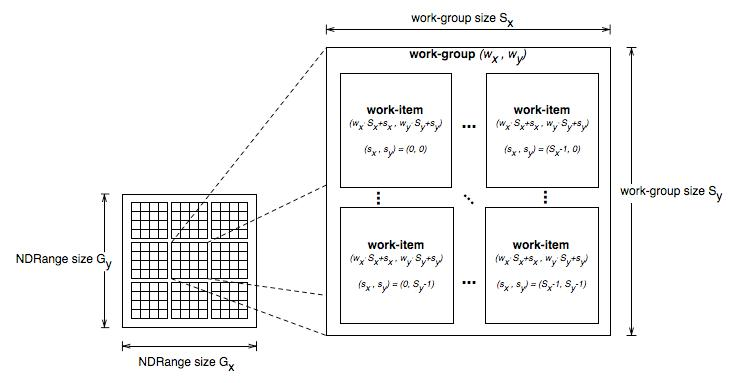
\includegraphics[width=\linewidth,height=\paperheight,keepaspectratio]{gpgpu.jpg}
	\caption{GPGPU Diagram}
	%Figure \ref{fig:gpgpuImg} shows our blockDiagram.
	\label{fig:gpu}
	\end{figure}
\pagebreak

\subsubsection{GPU Architecture Overview}
\paragraph{Specific designs of compute units can vary between GPUs but common components include:}
\begin{itemize}
\item Large groups of SIMD processors with separate private memory (registers) 
\item Local memory that is shared between the processors on a compute unit
\item Specialized components for pixel/texture operations such as rasterization
\item Global memory components such as a L1 cache (on the compute unit) and L2 cache that is accessible globally for all compute units.
\item Figure \ref{fig:gpuArch} shows an example compute unit design and Figure \ref{fig:gpuMem} shows the general memory model pattern.
\end{itemize}
	\begin{figure}[H]
	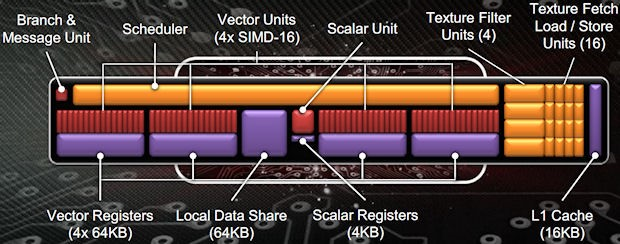
\includegraphics[width=\linewidth,height=\paperheight,keepaspectratio]{gpuArch.jpg}
	\caption{GPU Architecture Diagram}
	%Figure \ref{fig:gpgpuImg} shows our blockDiagram.
	\label{fig:gpuArch}
	\end{figure}
	
	\begin{figure}[H]
	\centerline{ 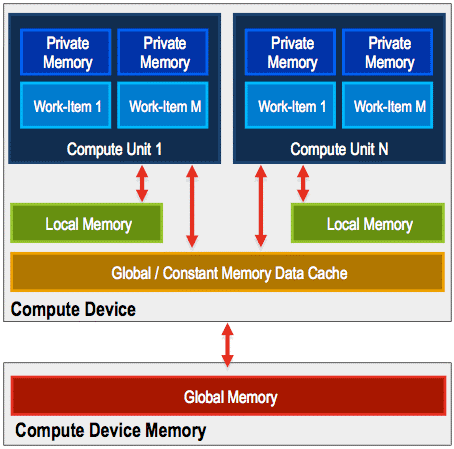
\includegraphics[scale=0.5]{gpuMem.png}}
	\caption{GPU Memory Diagram}
	%Figure \ref{fig:gpgpuImg} shows our blockDiagram.
	\label{fig:gpuMem}
	\end{figure}
\pagebreak



\subsubsection{Unity Support for Asynchronous Compute Shaders and Kenrels}
\paragraph{ Shading Languages used in Unity} ~\\
In Unity, shader programs are written in a variant of HLSL language (also called Cg but for most practical uses the two are the same). Unity recommneds developers have a good understanding 
of OpencL Or CUDA, OpenGL, and other Graphics/ GPGPU parallel compute languages.  

Internally, different shader compilers are used for shader program compilation:
\begin{itemize}
  \item Windows and Microsoft platforms (DX9, DX11, DX12, XboxOne and Xbox 360 ) all use Microsoft's HLSL compiler.
  \item OpenGL Core (GL3) and OpenGL ES 3 use Microsoft’s HLSL followed by bytecode translation into GLSL, using a modified version of hlslcc.
  \item OpenGL Legacy (GL2), OpenGL ES 2.0 and Metal use source level 
  translation via
  hlsl- 2glslfork and glsl optimizer. 
  \item Other console platforms use their respective compilers (e.g. PSSL on PS4).
  \item Surface Shaders use Cg 2.2 and MojoShader for code generation analysis step.
\end{itemize} %unity ref http://docs.unity3d.com/Manual/SL-ShadingLanguage.html
\subsubsection{Unity Cross Platfrom Shader Support (Android)}
In order to achieve shaders working on multiple different platforms one should consider these limitations:

\begin{itemize}
\item 
D3D and OpenGL have different data layout rules. Automatically translated GLSL shaders use std430 layout on compute buffers. Therefore for example using float3 based structured buffers will cause compatibility issues as DX allows tight packing but OpenGL enforces padding to float4. Scalars, two-component and four-component vectors are safe to use as they are. Extra care should be taken when constructing structs.
\item 
OpenGL ES 3.1 guarantees support for only 4 simultaneous shader storage buffers. Actual implementations typically support a bit more but in general one should consider grouping related data in structs as opposed to having each data item in its own buffer.
HLSL-only or GLSL-only compute shaders

\end{itemize}

Typically compute shader files are written in HLSL, and compiled or translated into all needed platforms automatically. However it is possible to either prevent translation to GLSL (i.e. only keep HLSL platforms), or to write GLSL compute code manually.
\begin{itemize}
\item Compute shader source surrounded by CGPROGRAM and ENDCG keywords will not be processed for OpenGL/GLSL platforms.
\item Compute shader source surrounded by GLSLPROGRAM and ENDGLSL keywords will be treated as GLSL source, and emitted verbatim. This will only work when targetting OpenGL/GLSL platforms.
\end{itemize}
\pagebreak

\subsubsection{Unity Support for Graphics Asset Related Operations}
One of the common bottlenecks in GPGPU processing is buffer transfer to the GPU memory before processing, Unity allows asynchronous texture uploads to allow the application to time slice the GPU resources to upload textures or other assets to the device, this means that it will take longer overall time to do transfer assets but if scheduled properly the background expected algorithms that need specific buffers should not have to block on the buffer transfers.
\begin{figure}[H]
	\centerline{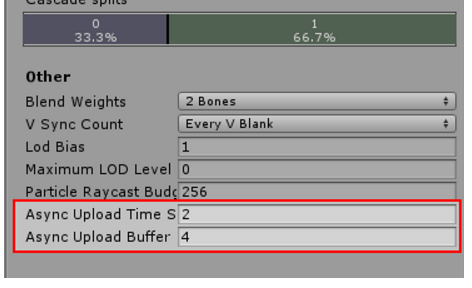
\includegraphics[scale= 0.75]{asychTexture.png}}
	\begin{itemize}
\item Upload time: Amount of time (ms) spent on asynchronous uploads per frame.
\item Upload Buffer: Size of texture upload buffer in MB unity usually adjusts this automatically but it can be set by the application.
\end{itemize}
	\caption{Unity Asynch Texture Options}
	%Figure \ref{fig:gpgpuImg} shows our blockDiagram.
	\label{fig:gpuTex}
	\end{figure}

\paragraph{Guarantees and Restrictions} 
For non-read/write enabled textures, the Texture Data is part of resS (Streaming Resource) and upload now happens on Render-Thread. Availability of Texture is guaranteed during call to AwakeFromLoad. (This only works for textures or buffers that are not used in any custom processing.)
~\\
For other types of texture loading, such as read/write enabled textures, textures loaded directly with the LoadImage(byte[] data) function, or loading from the Resources folder, the Asynchronous buffer loading is not used - the older Synchronous method is used.
These restrictions mean that we will have to schedule and synchronize the transfer of any custom textures or buffers to and from the GPU.
In order to avoid all of the transfer penalties the frequency, size, and amount of transfers should be minimized, and all the major assets should be kept on the GPU.

\pagebreak


\subsubsection{Unity Camera Rendering Pipeline}
Unity supports the exposes the command buffer which is similar to the main rendering pipeline in most graphics processing frameworks (OpenGL's paint or render loop, OpenCL's command queue etc.) This framework supports blitting, drawing meshes, drawing procedual geometry (compute shaders), and many other common graphics drawing features. \textbf{(See Figure \ref{fig:gpuPipe})}

\begin{figure}[H]
	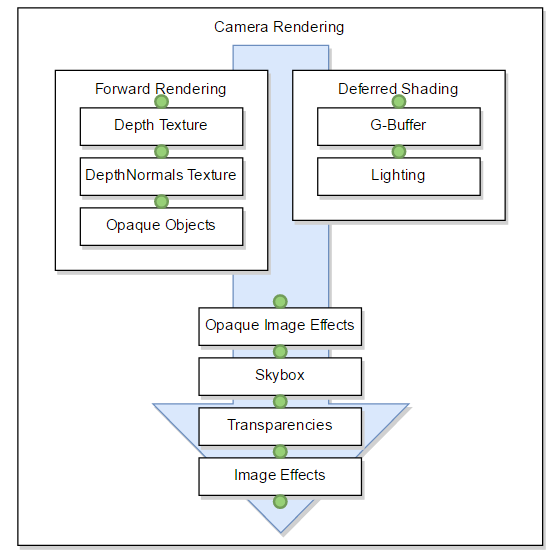
\includegraphics[width=\linewidth,height=\paperheight,keepaspectratio]{cameraRender.png}
	\caption{Unity Command Buffer Camera Pipeline}
	%Figure \ref{fig:gpgpuImg} shows our blockDiagram.
	\label{fig:gpuPipe}
	\end{figure}

\pagebreak

\subsubsection{Supported GPGPU Advanced features}
% try unity zip in google drive with atomic and local mem barriers
Some advanced GPGPU related constructs useful for highly optimized compute processing, need to be checked if they are included in Unity's implementation of DirectCompute,which 
is similar to the HLSL code snippets listed below.

\paragraph{Shared Memory Reduction Kernel}
\begin{figure}[H]
	\label{fig:reductionCode}
\lstinputlisting [language =C] {shared_mem_reduction.hlsl}
\caption{Reduction Code}
\end{figure}

This kernel is a computeShader that is run on the GPU and allows for synchronization of shared memory across multiple compute units, this technique is useful for parallel reduction algorithms which include
calcualtions such as min, max, mean, sum etc... anything that can be reduced to simpler worksets are are not itterative in nature. \textbf{(see figure \ref{fig:reductionImg})}

\begin{figure}[H]
	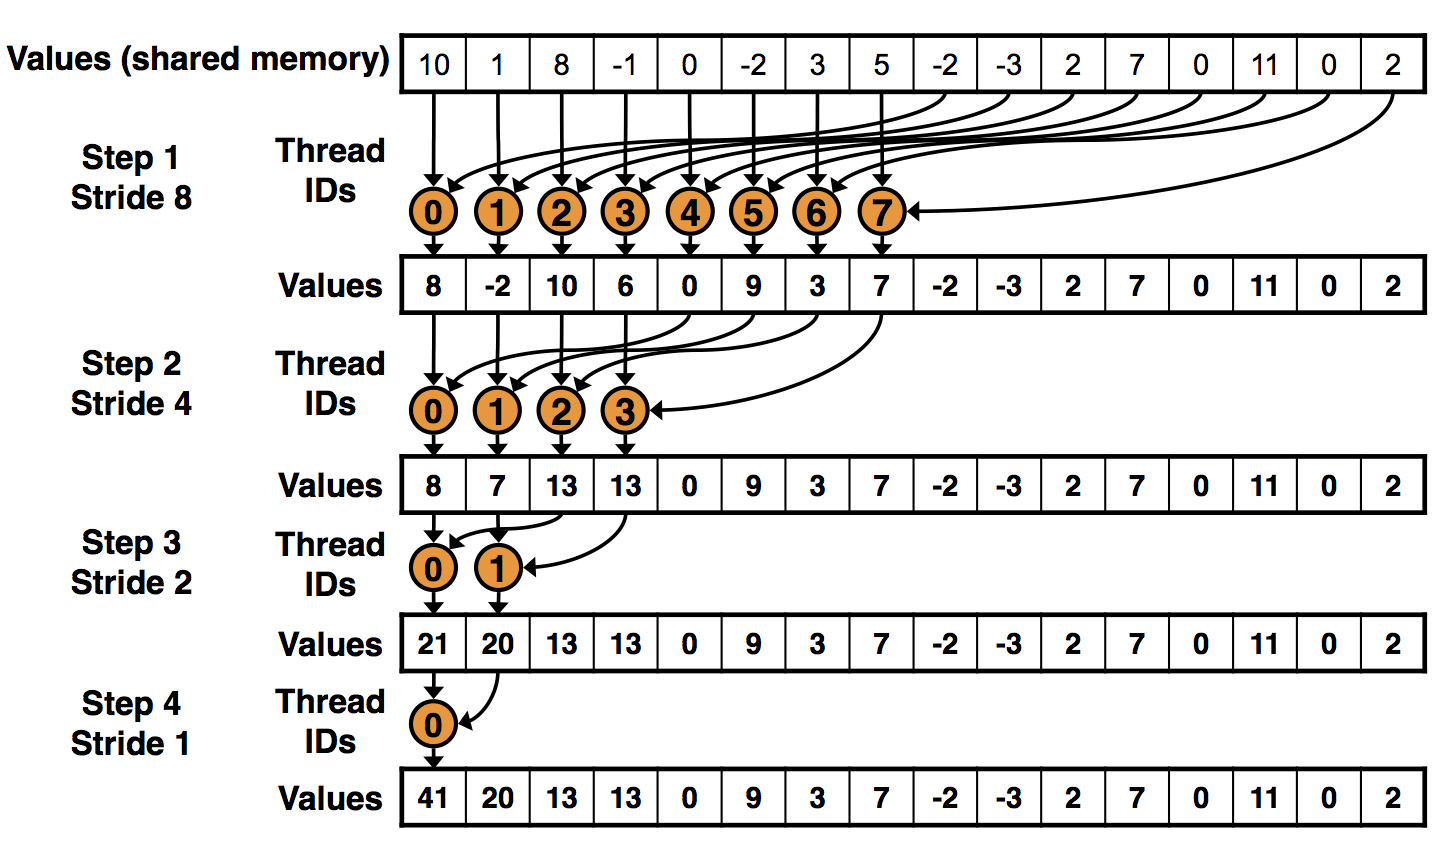
\includegraphics[width=\linewidth,height=\paperheight,keepaspectratio]{reduction.jpg}
	\caption{Reduction Diagram}
	%Figure \ref{fig:gpgpuImg} shows our blockDiagram.
	\label{fig:reductionImg}
	\end{figure}
\paragraph{Shader Processor Atomics} 
This is another powerful feature that is supported in Unity Compute shaders, it creates atomic accesses for compute units and shader processors which allow the kernels to avoid race conditions. 
\begin{figure}[H]
\lstinputlisting [language =C] {atomic_inc.hlsl}
This kernel is a compute shader that is run on the GPU and allows for synchronization adding or various operations that are done in an atomic fashion, avoiding, race conditions.
\caption{Atomic Code}
%Figure \ref{fig:gpgpuImg} shows our blockDiagram.
\label{fig:atomicCode}
\end{figure}

\pagebreak
%E. Explicit Design Summary with diagrams
%F. Build, prototype, test, and evaluation plan
\section{Design Documentation}
	\subsection{Block Diagrams:}
	\begin{figure}[H]
	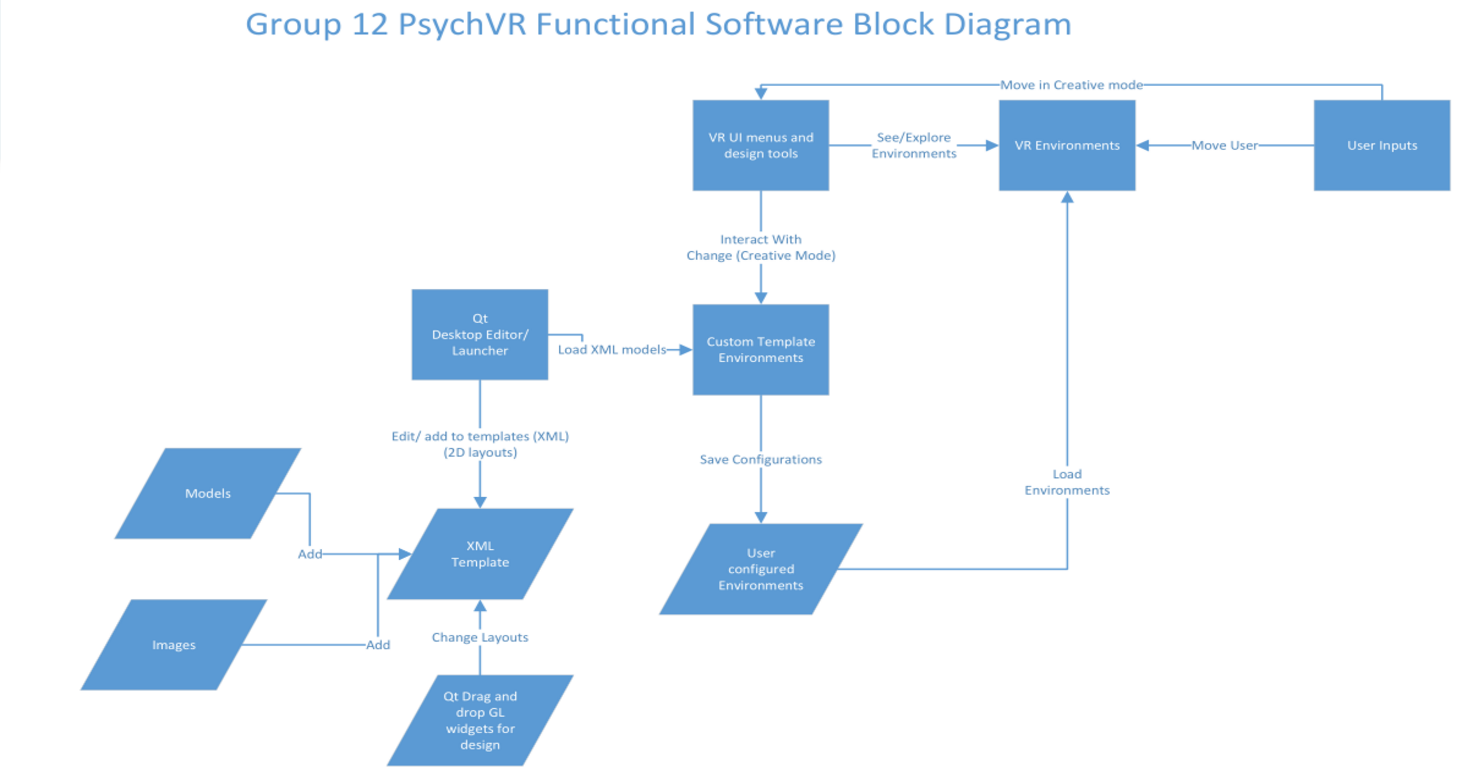
\includegraphics[width=\linewidth,height=\paperheight,keepaspectratio]{HardwareConfig.png}
	\caption{Hardware Block Diagram}
	%to ref fig number
	%Figure \ref{fig:block1} shows our blockDiagram.
	\label{fig:hblock}
	\end{figure}
	This diagram represents a hardware configuration of a typical VR system that our application would expect. This may change depending on the device we use, but is a good overview.
	\pagebreak
	\begin{figure}[H]
	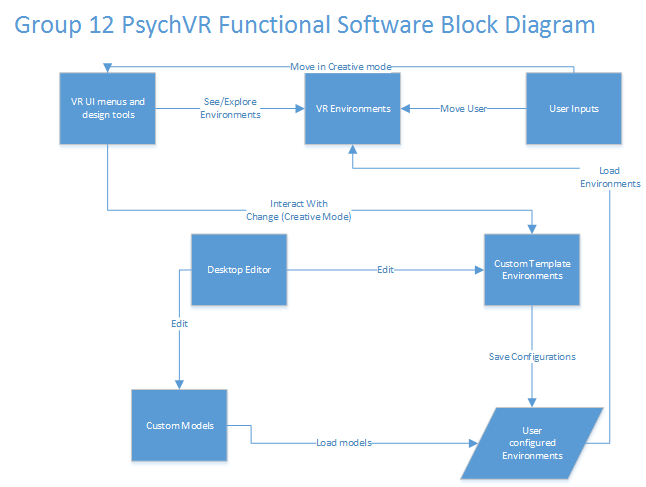
\includegraphics[width=\linewidth,height=\paperheight,keepaspectratio]{SoftwareConfig.png}
	\caption{Software Block Diagram}
	%to ref fig number
	%Figure \ref{fig:block2} shows our blockDiagram.
	\label{fig:sblock}
	\end{figure}
	This diagram represents the software design of our project and the various functional modules that should exist in order to fulfill the user interaction requirements. 
	The application will have two main modes of operation, edit mode and view mode. 
	\subsection{High Level Design}
		\begin{figure}[H]
			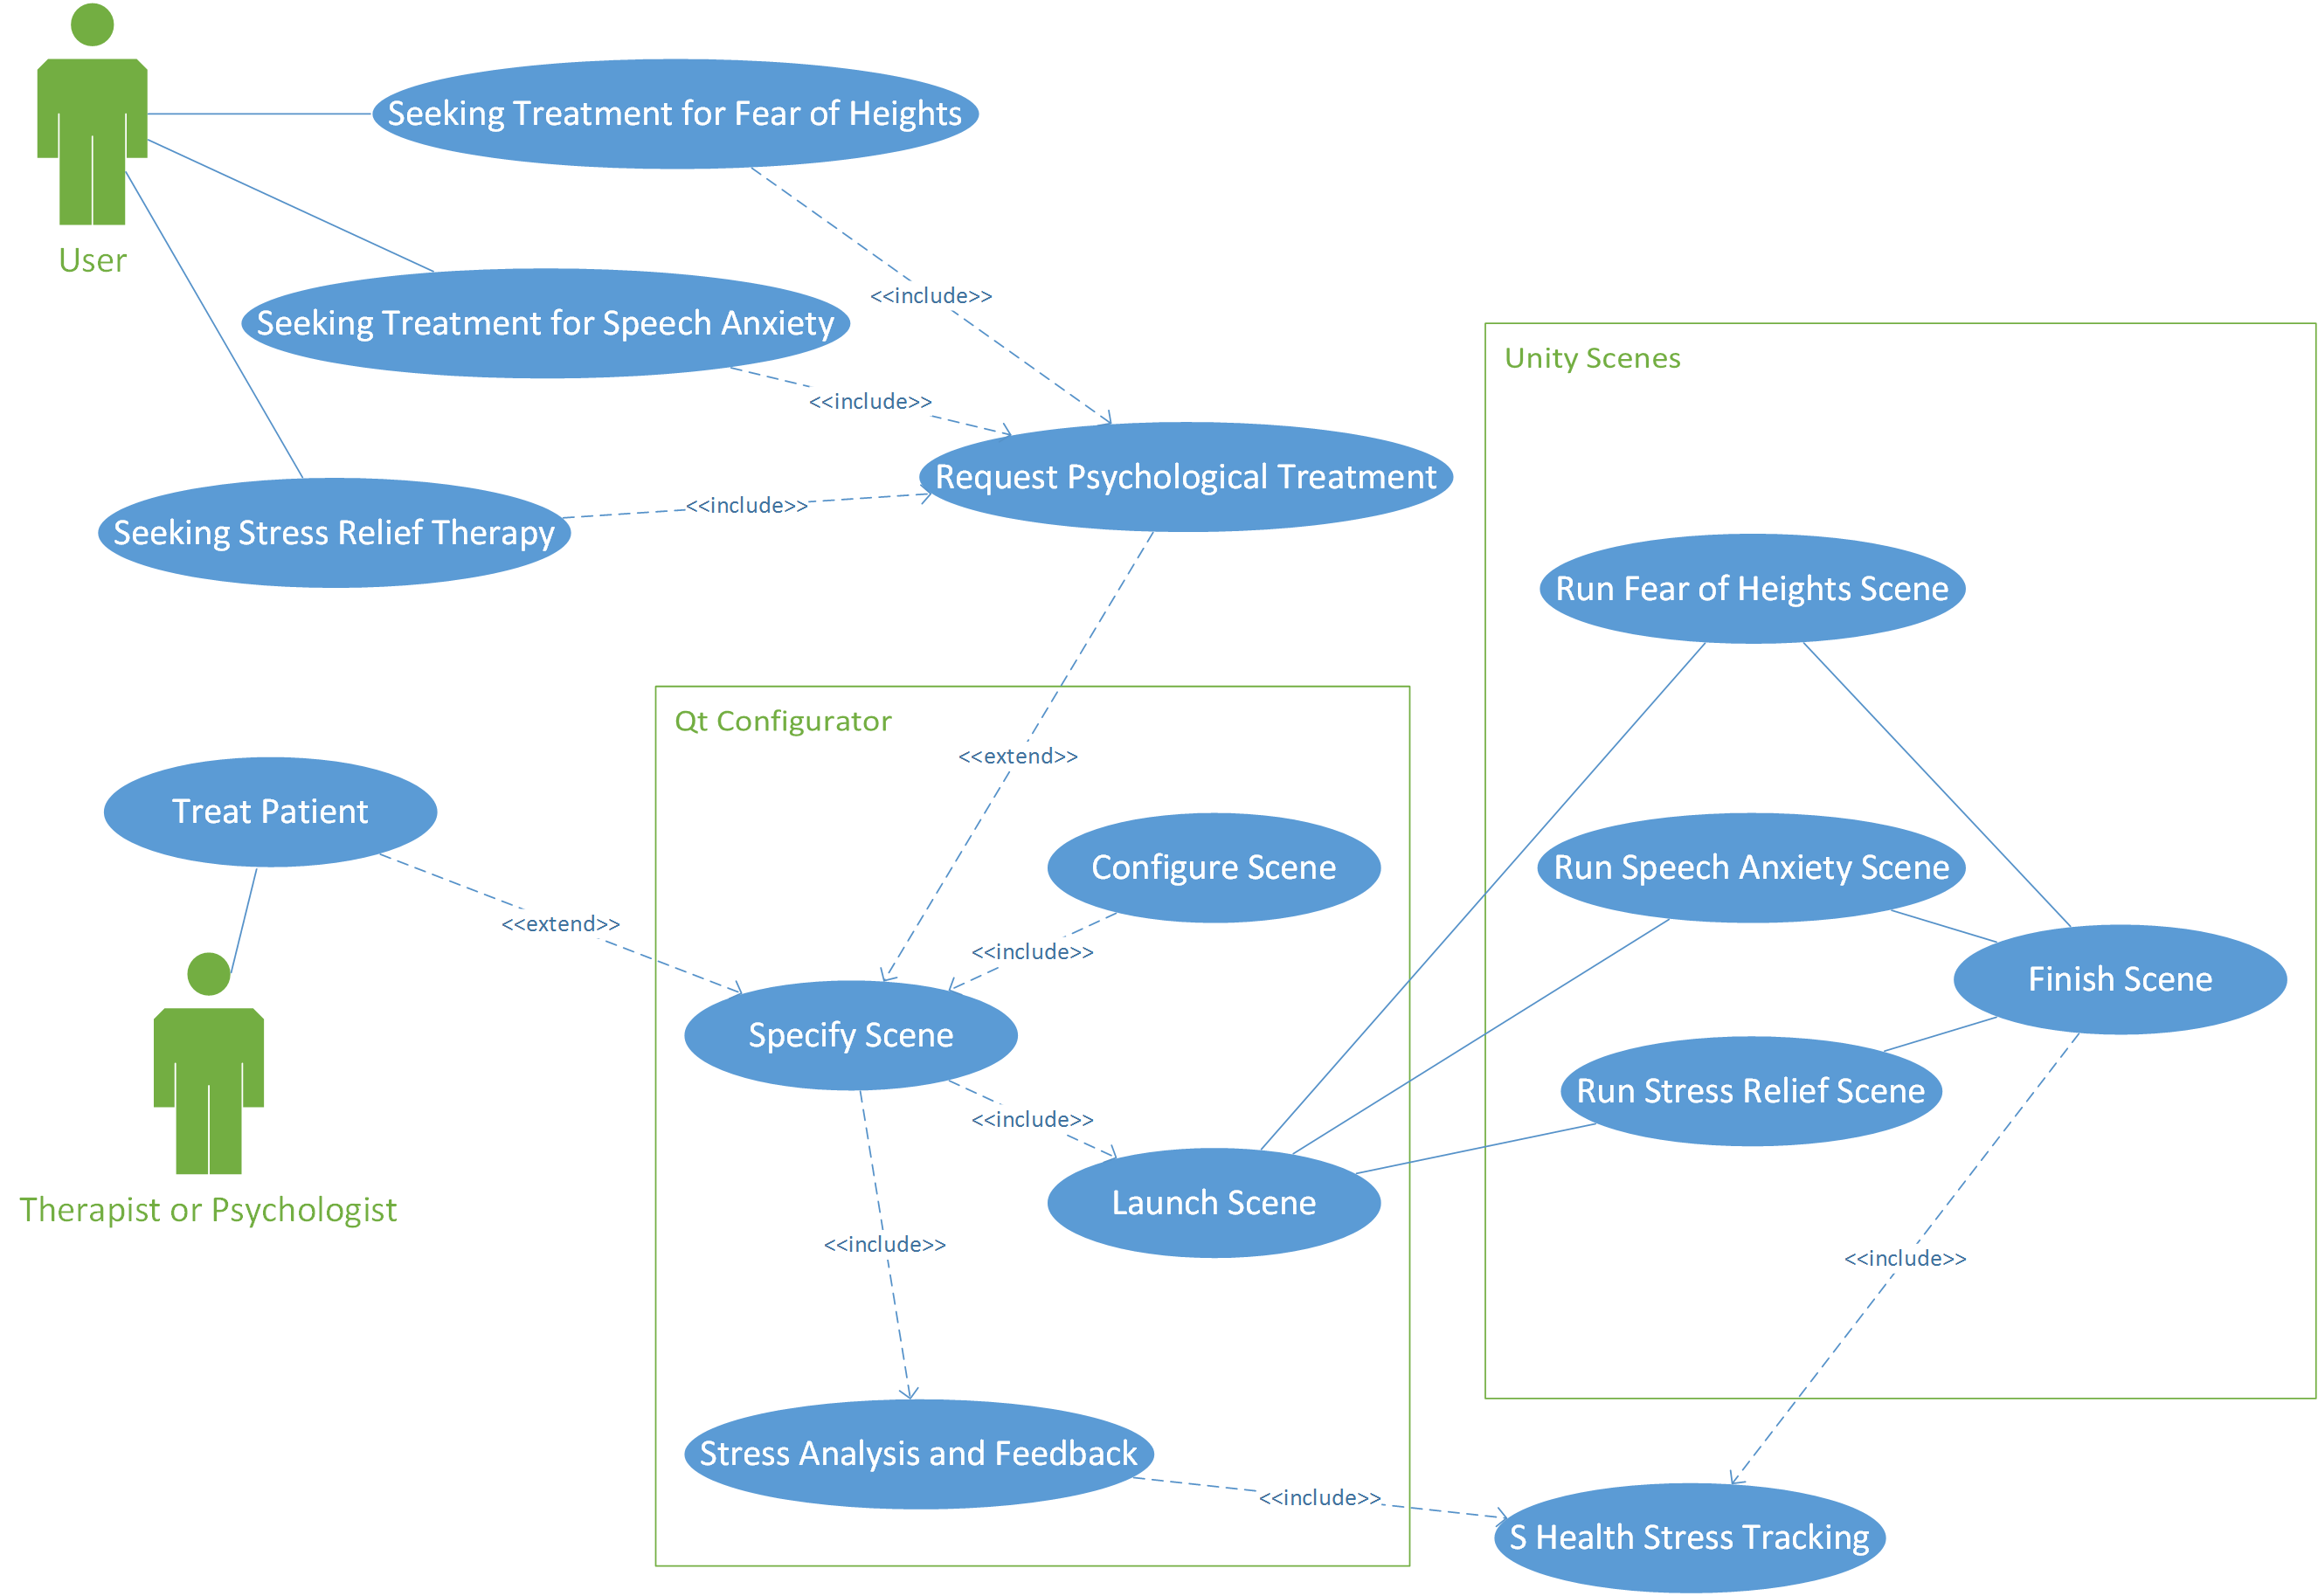
\includegraphics[width=\linewidth,height=\paperheight,keepaspectratio]{highUseCase.png}
			\caption{High Level Use Case Diagram}
			%to ref fig number
			%Figure \ref{fig:block2} shows our blockDiagram.
			\label{fig:highlevelusecase}
		\end{figure}
	\pagebreak
	\subsection{Qt Design Plan}
		\subsubsection{High Level Diagram}
		\pagebreak
		\subsubsection{Activity Diagram}
				\begin{figure}[H]
					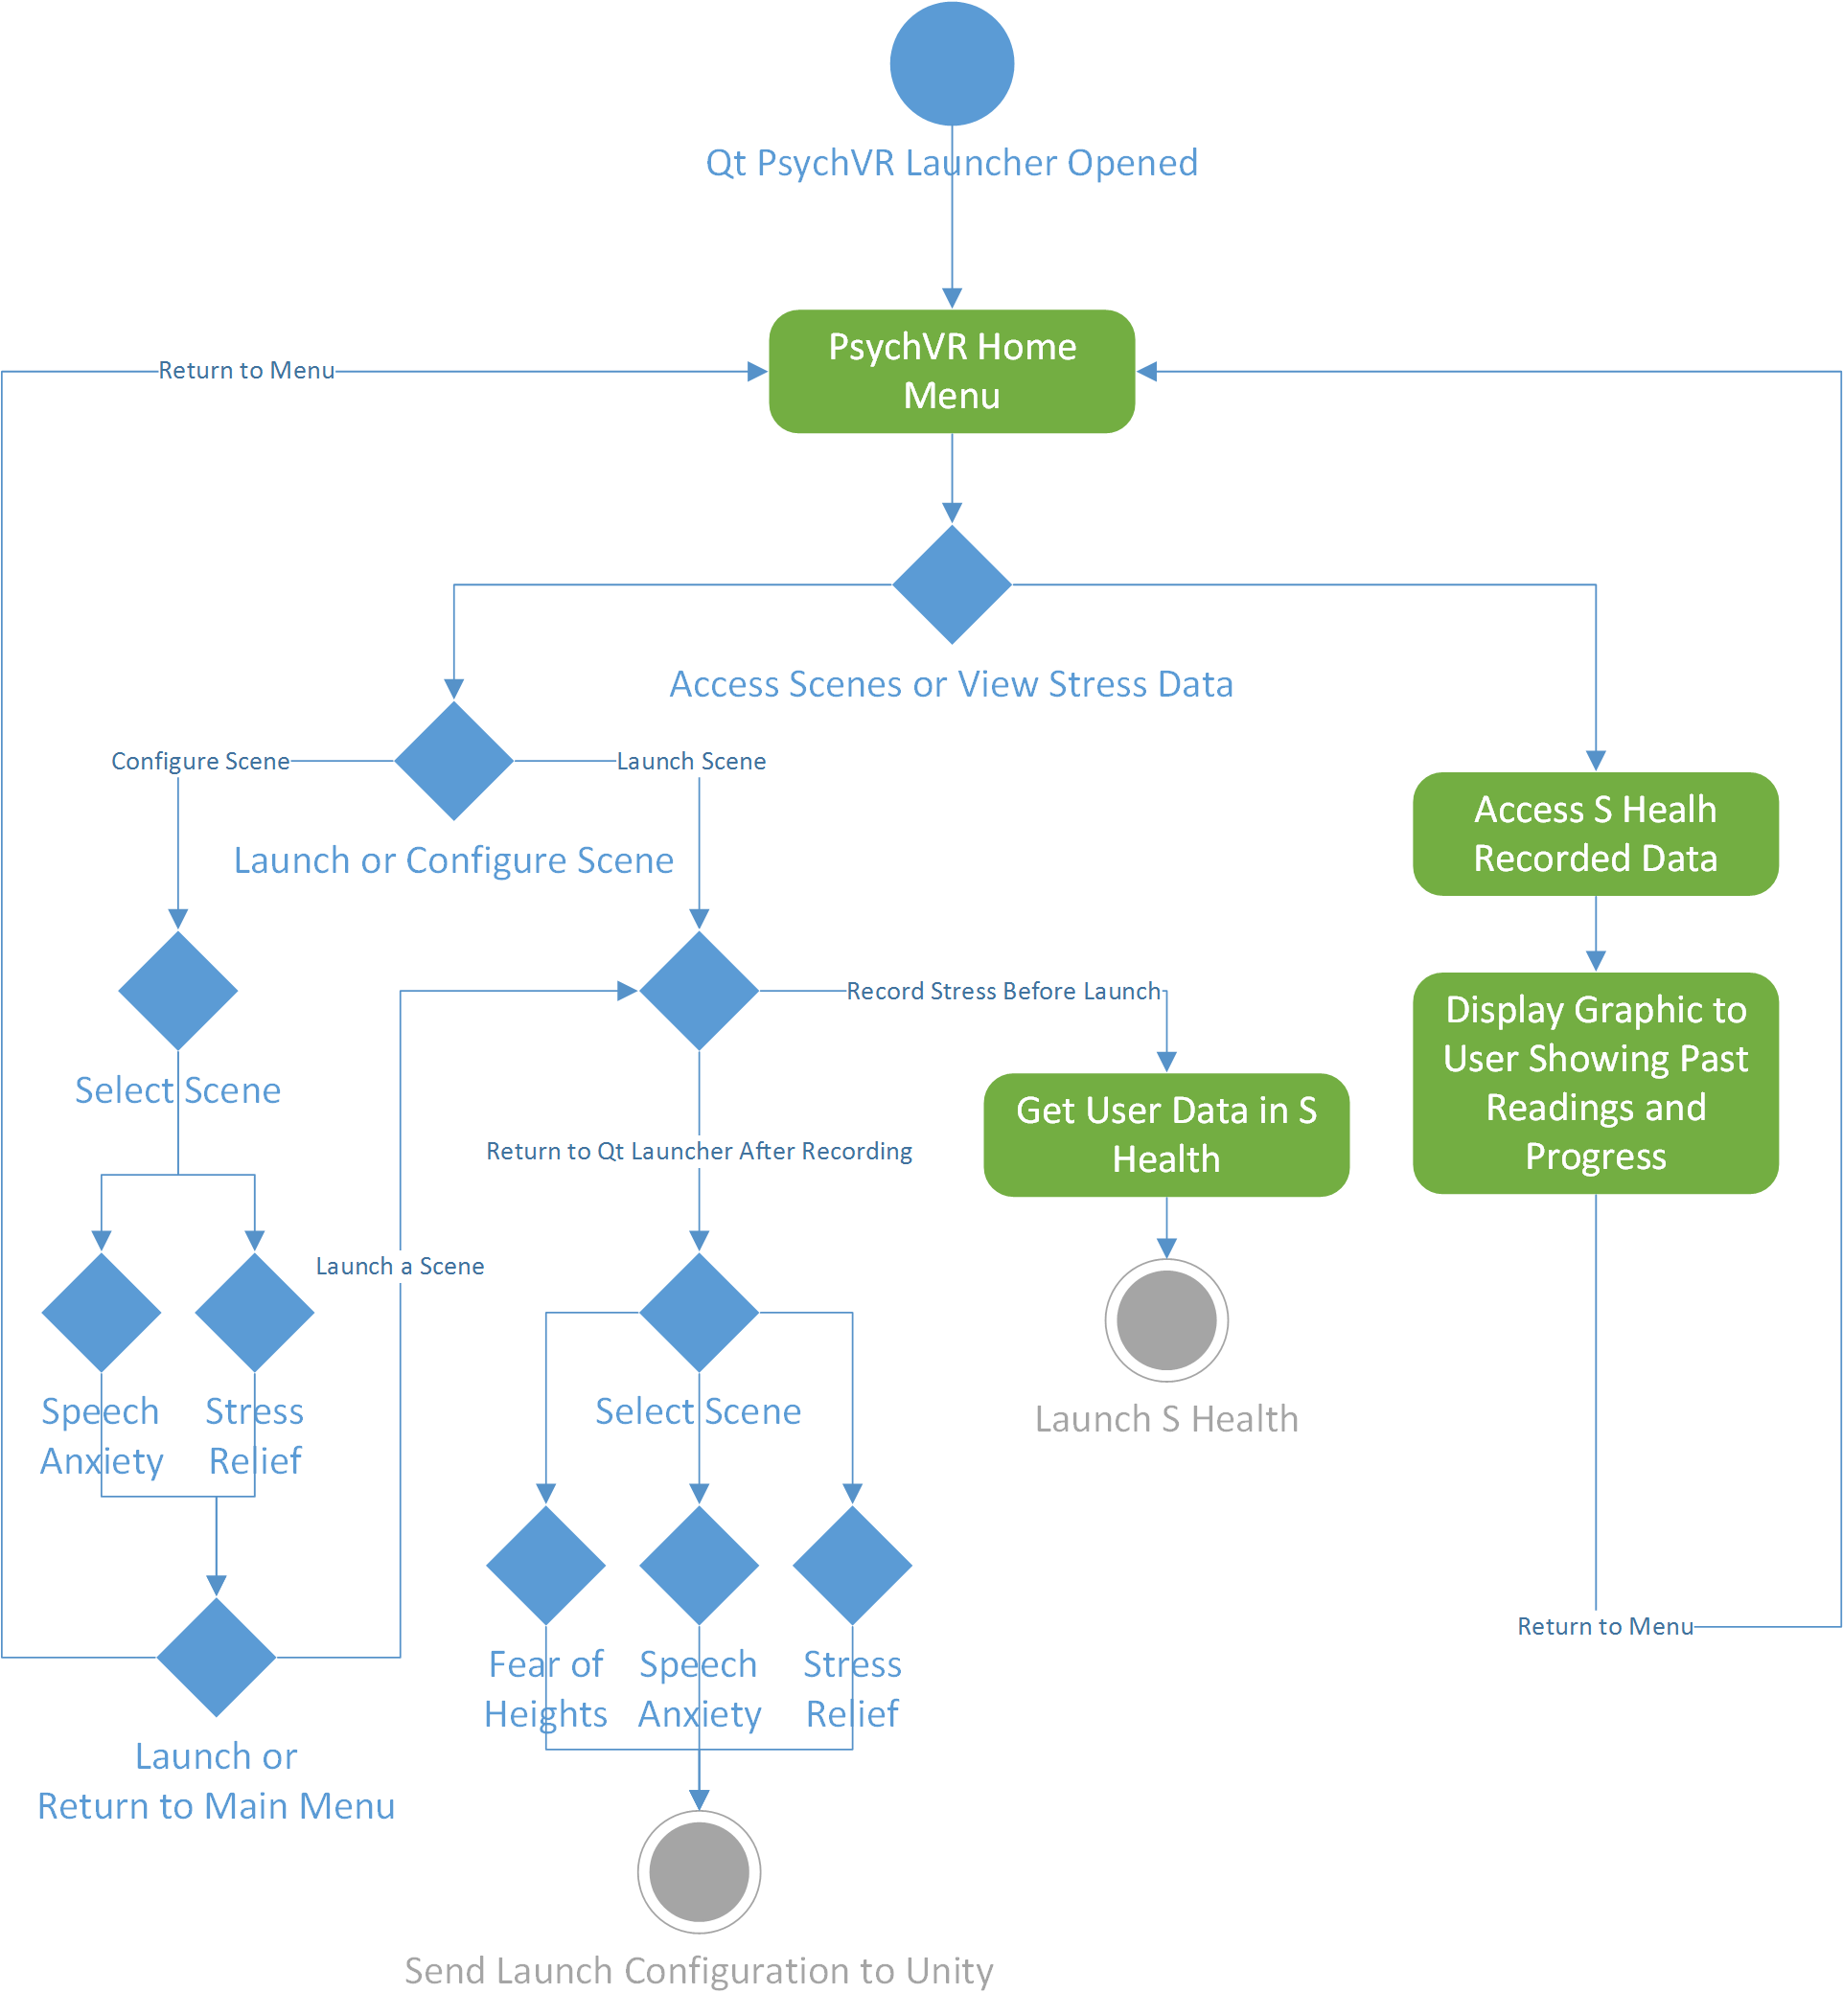
\includegraphics[width=\linewidth,height=\paperheight,keepaspectratio]{qtActivityDiag.png}
					\caption{Qt Activity Diagram}
					%to ref fig number
					%Figure \ref{fig:block2} shows our blockDiagram.
					\label{fig:qtactivity}
				\end{figure}
				\pagebreak
	\subsection{Unity Hierarchy}
		\subsubsection{High Level Design}
		\pagebreak
		\subsubsection{Activity Diagram}
				\begin{figure}[H]
					\centerline{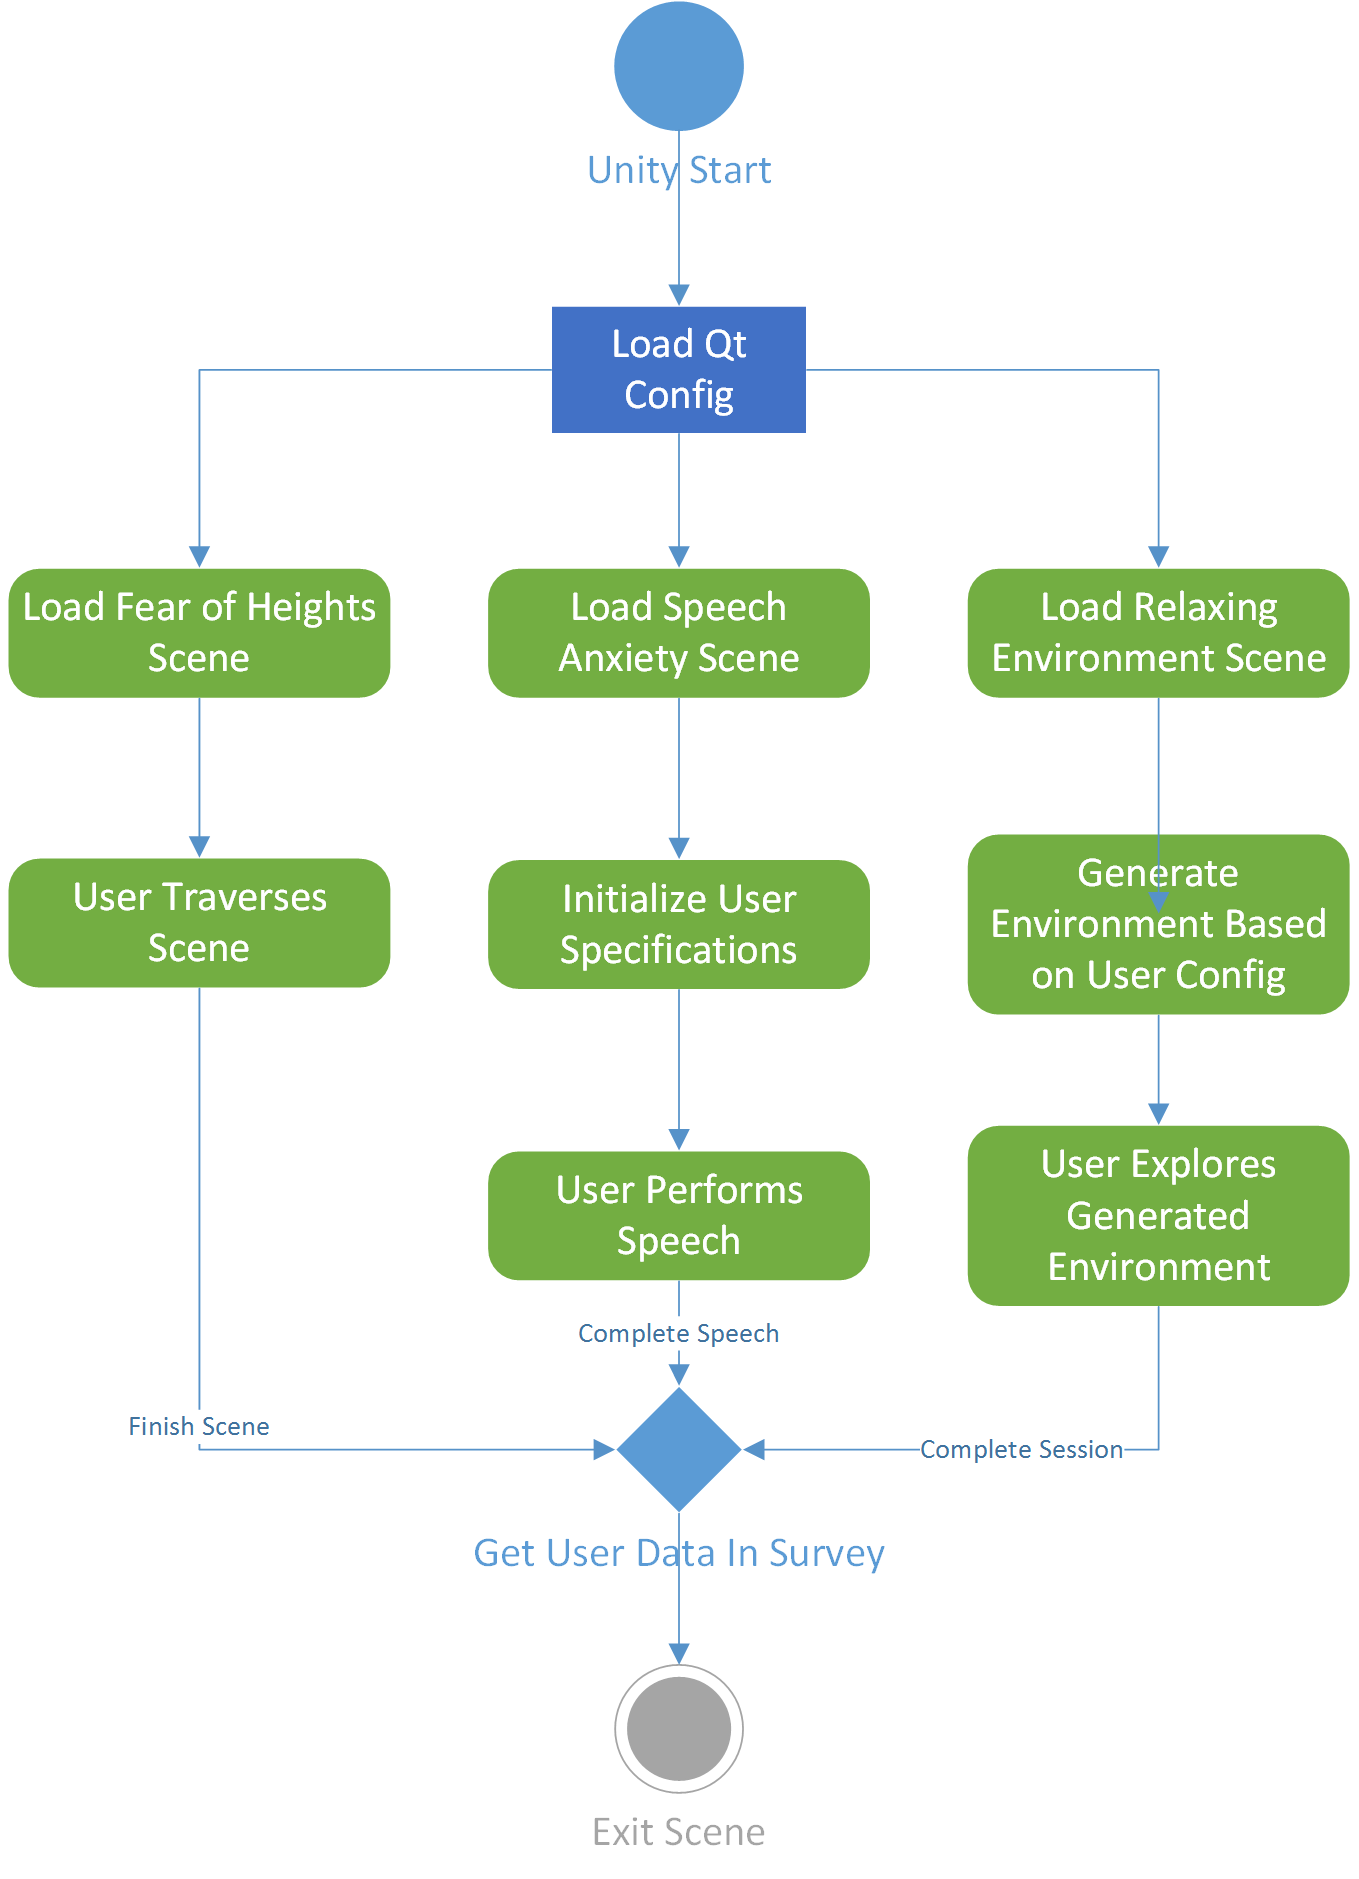
\includegraphics[]{unityActivityDiag.png}}
					\caption{Unity Activity Diagram}
					%to ref fig number
					%Figure \ref{fig:block2} shows our blockDiagram.
					\label{fig:unityactivity}
				\end{figure}
				\pagebreak
		\subsubsection{Scene Shared Assets}
	\subsection{Test Plan}

\pagebreak

%4. Administrative content
%G. Personnel and bibliography of related work, if any (mostly text)
%H. Facilities and Equipment (text, numbers, tables, charts, figures, diagrams)
%I. Consultants, subcontractors, and suppliers (mostly text)
%A. Budget and financing (text, numbers, tables, charts, figures, diagrams).
%B. Milestone chart for all activities related to the project
\section{Administrative Content}
\section{Budget and Financing}
			    Financing is still being researched at this point.  Due to us not having a sponsor, we will either have to self-finance or contact people willing to help with funding.  Therefore, our budget and financing are extremely subject to change. We already have the hardware necessary to run virtual reality hardware, so that saves us the cost of building one ourselves (upwards of 1000 dollars). VR headsets vary in price, although our current target the Oculus Rift, costs 600 dollars. Using Unity Pro costs 75 dollars a month, so over the next 8 months it would add up to another 600 dollars. This totals to 1200 dollars for development and hardware. However, a number of on campus facilities also have virtual 
			    reality headsets for testing and design purposes, including Sony’s VR headset Morpheus and a few Oculus Rifts.  If we can gain access to these facilities, we can cut down on hardware costs tremendously.  Additionally, if we can gain a sponsor or funding from UCF, we could potentially up our budget and invest in some newer VR 
			    technology, and possibly be able to test for multiple platforms. The upper limit would be the Microsoft Hololens, which costs between 1500 dollars and 3000 dollars for a dev kit, while it is something we would 
			    not be able to afford for this project alone, it could be something UCF would be interested in investing in.  
			    
			    \subsection{Summary:}
			    Current Budget: Roughly \$1500.  \$600 for Dev Kit,
			    \$600 for development Engine, \$200 for equipment and other software (in engine models, non-vr hardware such as controllers and cameras),\$100 for other
			    expenses that could come up.
			    
			    \subsection{Funding}
			    This is entirely self funded at the moment.  All of us have well-paying jobs in the 
			    Orlando area, and would be able to spend \$500 if necessary.  However, hopefully we will be able to at the very least cut out the 
			    \$600 Oculus Rift Dev Kit cost by using UCF facilities, and possibly cutting away the \$600 engine cost as well by settling on the limited free version of Unity.  
	%software licensing costs, cloud based service costs, code repo's, graphic design costs
	\section{Schedule}
	\begin{figure}[H]
	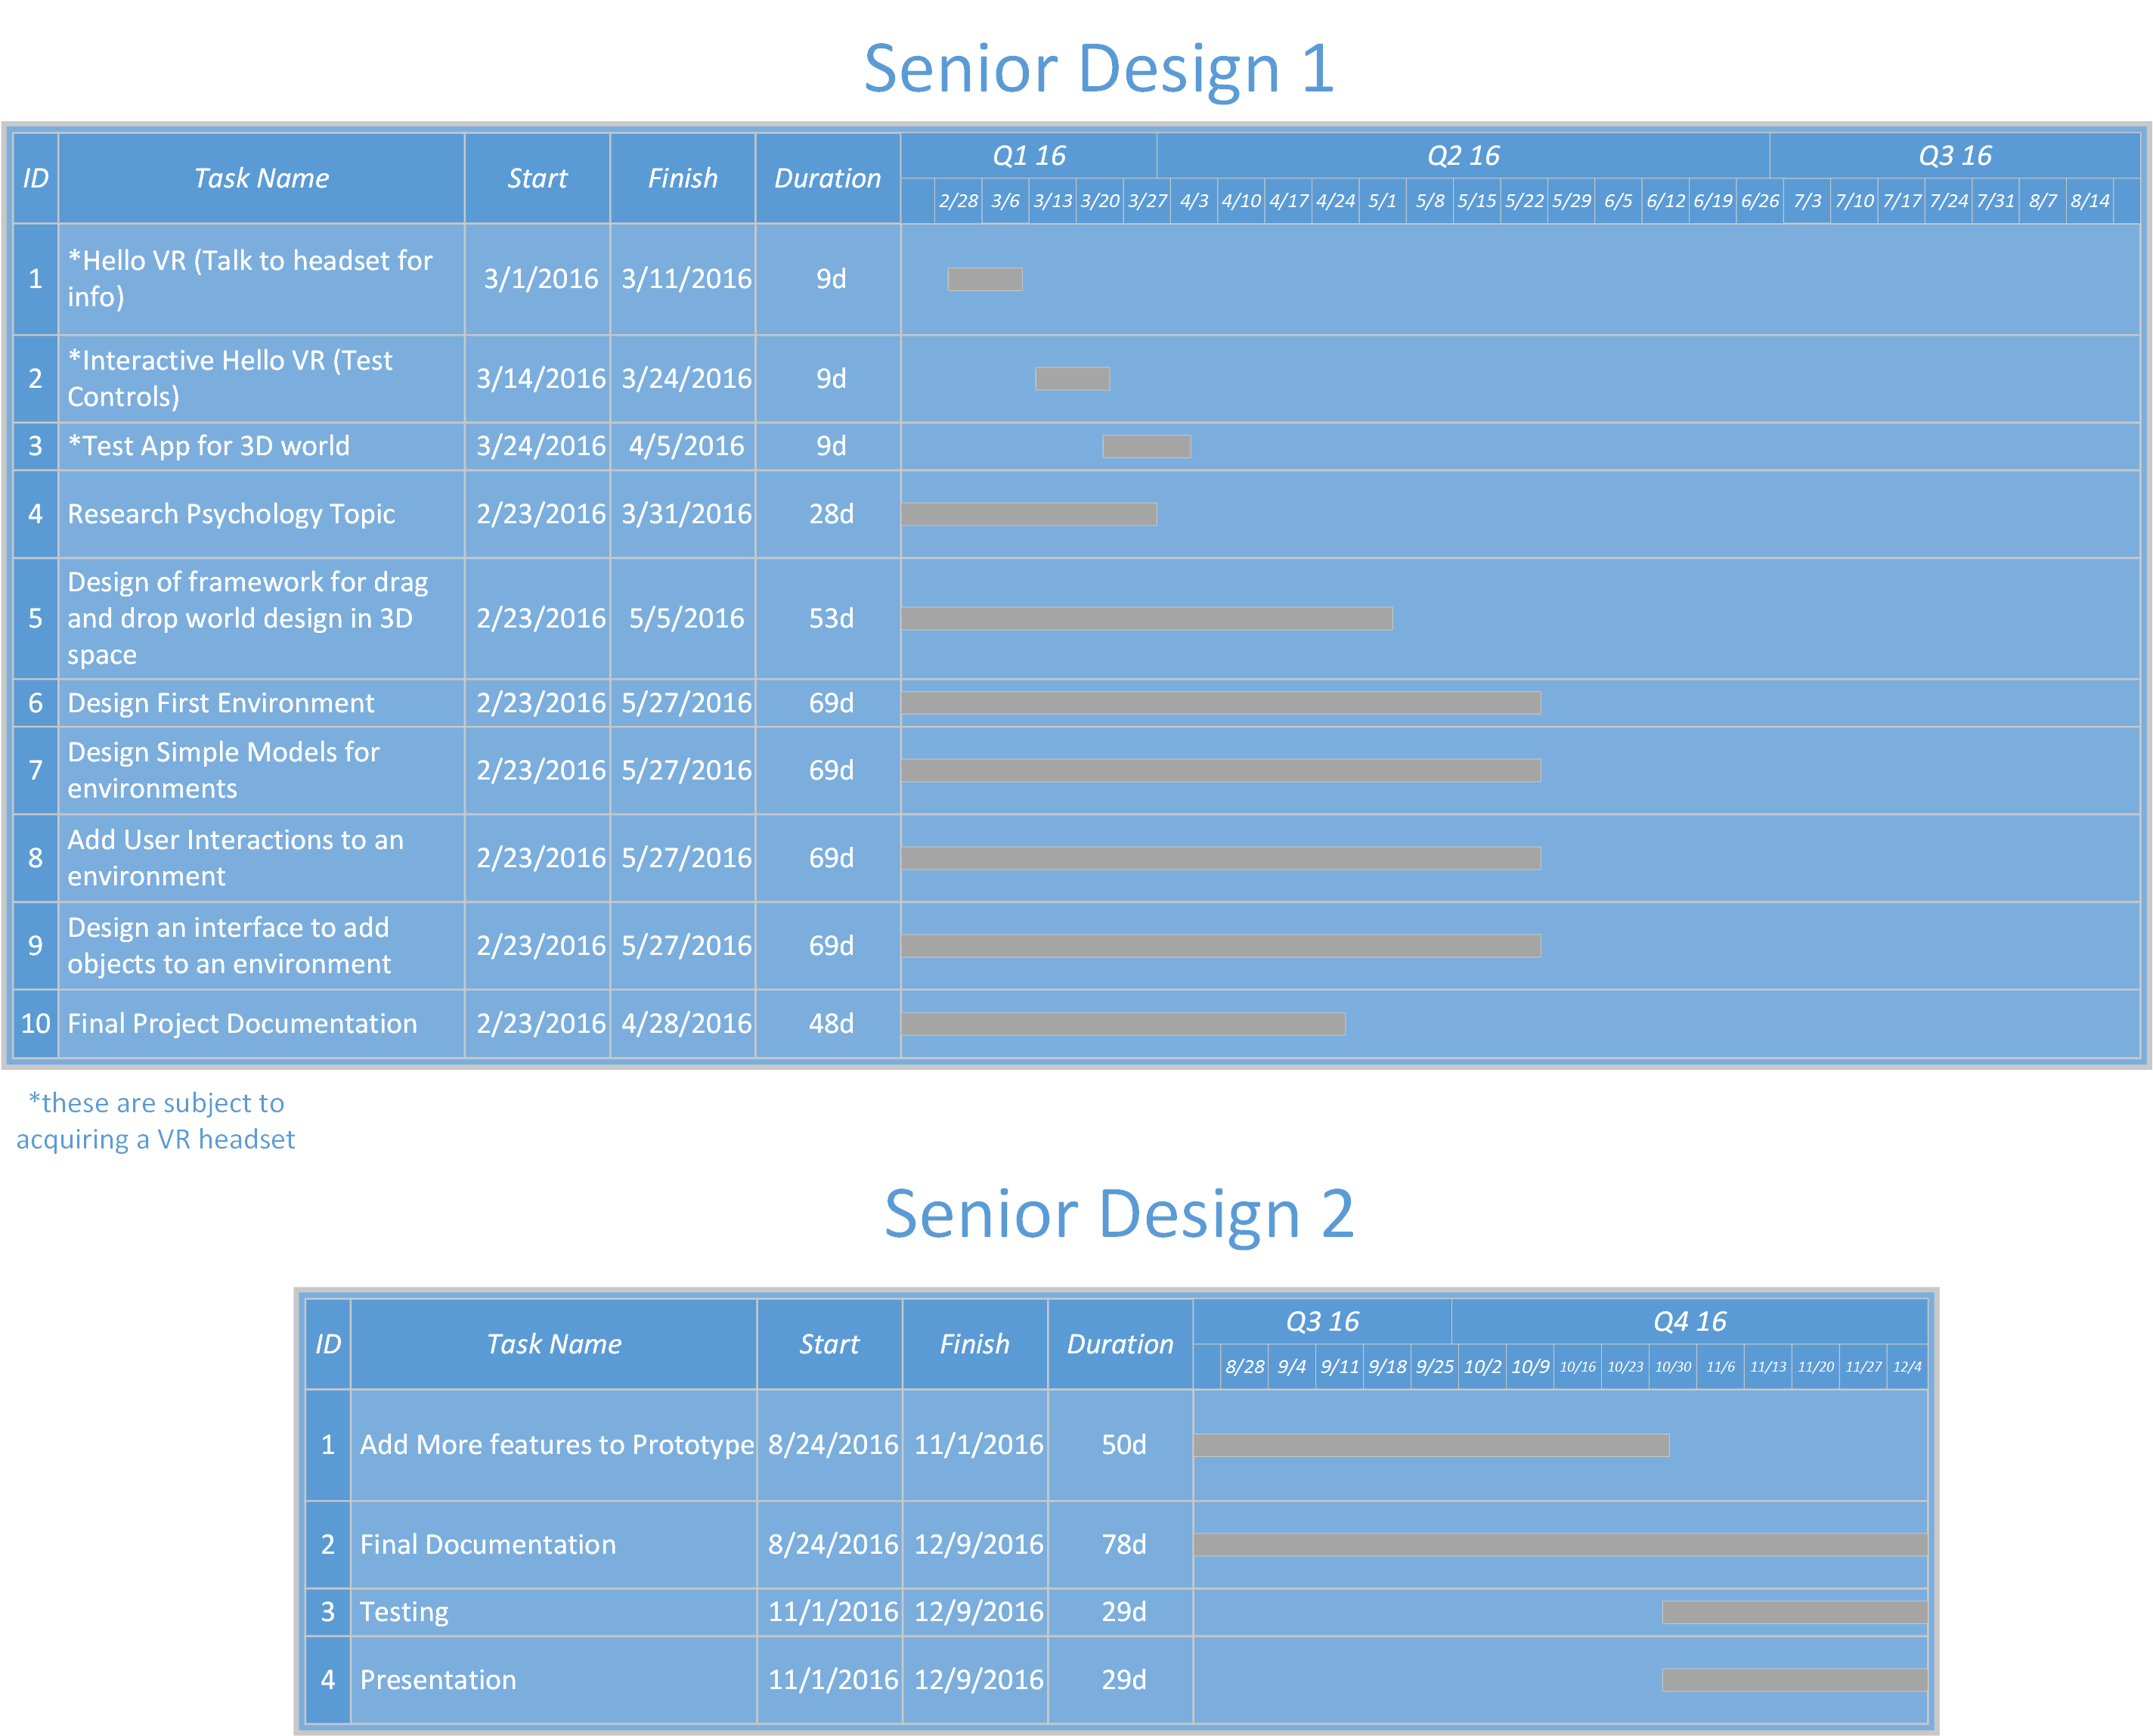
\includegraphics[width=\linewidth]{scheduleSR.png}
	\caption{Prototype Phase Gantt Chart:}
	%to ref fig number
	%Figure \ref{fig:block1} shows our blockDiagram.
	\label{fig:pchart}
	\end{figure}
	\section{Milestones}
	\subsection{Tech Milestones}
		\begin{itemize}
			\item Finding funding or available UCF facilities
			\item Obtaining Oculus Rift
			\item Obtaining Gear VR
			\item Obtaining LeapMotion
			\item Getting virtual reality hardware to display world
			\item Connecting user input to world
		\end{itemize}
	\subsection{Research Milestones}
		\begin{itemize}
			\item Choose the most important scenes to develop
			\item Testing with psychologists to confirm project is beneficial
		\end{itemize}
	\subsection{Development Milestones}
		\begin{itemize}
			\item Allowing for users to add models to world, and design said world
			\item Combining all aspects of project into cohesive whole
			\item Finalize and begin testing of project
		\end{itemize}
	
	%\subsection{Overall Milestones}
	%	\begin{itemize}
	%		\item get a decent amount of sleep,
	%               \item not procrastinate this hard on a paper again
	%		\item try not to cry
	%	\end{itemize}

\pagebreak
%5. Project Summary and conclusions.
\section{Project Summary and Conclusions}

\pagebreak
\pagenumbering{Alph}
\setcounter{page}{1}
%6. References
\section{References}

\bibliographystyle{mla}
\begin{thebibliography}{9}
\bibitem{stroke1}
Rettner, Rachael. "Stroke Therapy Gets Boost from Virtual Reality." LiveScience. TechMedia Network, 07 Apr. 2011. Web. 06 Apr. 2016.
\bibitem{dsmCaution}
"Cautionary Statement for DSM IV - TR." Cautionary Statement for DSM IV. N.p., n.d. Web. 10 Apr. 2016.
\bibitem {dsmPhobia}
"Diagnostic Criteria for 300.29 Specific Phobia." Diagnostic Criteria for 300.29 Specific Phobia. N.p., n.d. Web. 10 Apr. 2016.
\end{thebibliography}

%7. Appendices
\section{Appendices}

%A. Copyright permissions
\section{Copyright Permissions}

%B. Data-sheets (if necessary)
%C. Software (if necessary)
%D. Other
\section{Extras}

\end{document}
